% file: chap6.tex

\chapter{深度学习}
\label{ch:Deeplearning}

在\hyperref[ch:WhyHardToTrain]{上一章},我们学习了深度神经网络通常比浅层神经网络
更加难以训练。我们有理由相信,若是可以训练深度网络,则能够获得比浅层网络更加强大
的能力,但是现实很残酷。从上一章我们可以看到很多不利的消息,但是这些困难不能阻止
我们使用深度神经网络。本章,我们将给出可以用来训练深度神经网络的技术,并在实战中
应用它们。同样我们也会从更加广阔的视角来看神经网络,简要地回顾近期有关深度神经网
络在图像识别、语音识别和其他应用中的研究进展。然后,还会给出一些关于未来神经网络
又或人工智能的简短的推测性的看法。

这一章比较长。为了更好地让你们学习,我们先粗看一下整体安排。本章的小节之间关联并
不太紧密,所以如果读者熟悉基本的神经网络的知识,那么可以任意跳到自己最感兴趣的部
分。

\hyperref[sec:convolutional_networks]{本章主要的部分}是对最为流行神经网络之一的
深度卷积网络的介绍。我们将细致地分析一个使用卷积网络来解决 MNIST 数据集的手写数
字识别的例子(包含了代码和讲解):
\begin{center}
  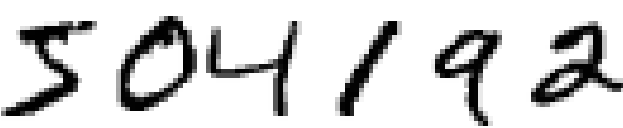
\includegraphics[width=64pt]{digits}
\end{center}

我们将从浅层的神经网络开始来解决上面的问题。通过多次的迭代,我们会构建越来越强大
的网络。在这个过程中,也将要探究若干强大技术:卷积、\gls*{pooling}、使用 GPU 来
更好地训练、训练数据的算法性扩展(避免\gls*{overfitting})、\gls*{dropout}技术的
使用(同样为了防止\gls*{overfitting}现象)、网络的综合使用和其他技术。最终的结果
能够接近人类的表现。在 10,000 幅 MNIST 测试图像上~——~模型从未在训练中接触的图
像~——~该系统最终能够将其中 9,967 幅正确分类。这儿我们看看错分的 33 幅图像。注意
正确分类是右上的标记;系统产生的分类在右下:
\begin{center}
  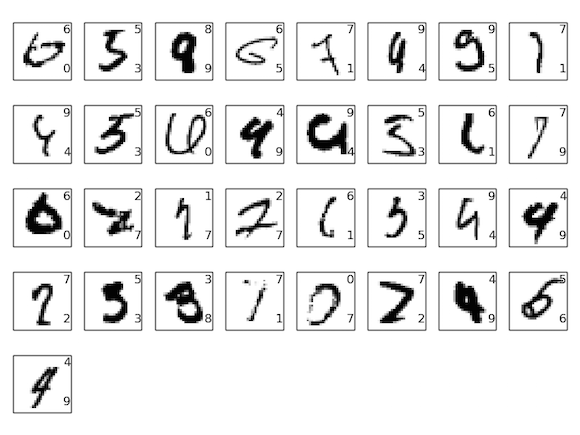
\includegraphics[width=.75\textwidth]{ensemble_errors}
\end{center}

可以发现,这里面的图像即使对于人类来说都是非常困难区分的。例如,在第一行的第三幅
图。我看的话,看起来更像是 “9” 而非 “8”,而 “8” 却是给出的真实的结果。我们
的网络同样能够确定这个是 “9”。这种类型的“错误”最起码是容易理解的,可能甚至值
得我们赞许。最后用对最近使用深度(卷积)神经网络在图像识别上的研究进展作为关于图
像识别的讨论的总结。

本章剩下的部分,我们将会从一个更加宽泛和宏观的角度来讨论深度学习。概述一些神经网
络的其他模型,例如\gls*{rnn}和\gls*{lstm},以及这些网络如何在语音识别、自然语言
处理和其他领域中应用的。最后会试着推测一下,神经网络和深度学习未来发展的方向,会
从\gls*{idui}谈谈深度学习在人工智能的角色。这章内容建立在本书前面章节的基础之上,
使用了前面介绍的诸如\gls*{bp}、\gls*{regularization}、\gls*{softmax-func},等等。
然而,要想阅读这一章,倒是不需要太过细致地掌握前面章节中内容的所有的细节。当然读
完第一章关于神经网络的基础是非常有帮助的。本章提到第二章到第五章的概念时,也会在
文中给出链接供读者去查看这些必需的概念。

需要注意的一点是,本章所没有包含的那一部分。这一章并不是关于最新和最强大的神经网
络库。我们也不是想训练数十层的神经网络来处理最前沿的问题。而是希望能够让读者理解
深度神经网络背后核心的原理,并将这些原理用在一个 MNIST 问题的解决中,方便我们的
理解。换句话说,本章目标不是将最前沿的神经网络展示给你看。包括前面的章节,我们都
是聚焦在基础上,这样读者就能够做好充分的准备来掌握众多的不断涌现的深度学习领域最
新工作。本章仍然在Beta版。期望读者指出笔误,bug,小错和主要的误解。如果你发现了
可疑的地方,请直接联系 mn@michaelnielsen.org。

\section{介绍卷积网络}
\label{sec:convolutional_networks}

在前面的章节中,我们教会了神经网络能够较好地识别手写数字:
\begin{center}
  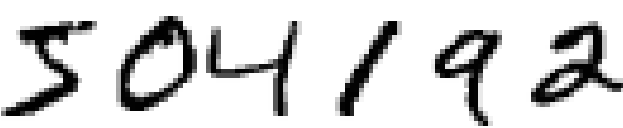
\includegraphics[width=64pt]{digits}
\end{center}

我们使用了全连接的邻接关系的网络来完成这个工作。即,网络中的神经元与相邻的层上的
每个神经元均连接:
\begin{center}
  \includegraphics{tikz41}
\end{center}

特别地,对输入图像中的每个像素点,我们将其光强度作为对应输入层神经元的值。对于
$28 \times 28$ 像素的图像,这意味着我们的网络有 784($= 28 \times 28$)个输入神
经元。我们然后训练网络的\gls*{weight}和\gls*{bias},使得网络输出能够~——~如我们希望地~——~正确地辨
认输入图像:'0', '1', '2', $\ldots$, '8', 或 '9'。

我们之前的网络工作得相当好:我们已经\hyperref[98percent]{得到了超过 98\% 的分类
  准确率},使用来自 \hyperref[sec:learning_with_gradient_descent]{MNIST 手写数字
  数据集}的训练和测试数据。但是仔细推敲,使用全连接层的网络来分类图像是很奇怪的。
原因是这样的一个网络架构不考虑图像的空间结构。例如,它在完全相同的基础上去对待相
距很远和彼此接近的输入像素。这样的空间结构的概念必须从训练数据中推断。但是如果我
们使用一个设法利用空间结构的架构,而不是从一个\textbf{白板状态}的网络架构开始,
会怎样?在这一节中,我会描述\textbf{\gls{cnn}}\footnote{最初的\gls*{cnn}要追溯到
  1970 年代。但是建立起现代卷积网络学科的开创性论文是一篇1998 年的
  “\href{http://yann.lecun.com/exdb/publis/pdf/lecun-98.pdf}{Gradient-based
    learning applied to document recognition}”,作者为 Yann LeCun, Léon
  Bottou, Yoshua Bengio, 和 Patrick Haffner。LeCun 自那以后做了一个关于卷积网
  络术语的有趣评论:“以类似卷积网络模型的[生物学上的]神经系统原型是非常牵强的。
  这正是为什么我把它们称为‘卷积网络’而不是‘\gls*{cnn}’,以及为什么我们称这些
  节点为‘单元’而不是‘神经元’”。尽管有这样的评论,卷积网络使用许多我们目前为
  止学习到的神经网络相同的思想:诸如反向传播,梯度下降,\gls*{regularization},
  非线性激活函数等等。所以我们会遵循常规惯例,认为它们是神经网络的一种类型。我会
  交换地使用术语“\gls*{cnn}”和“卷积网络(行为)”。我也会交换地使用术语“[人
    工]神经元”和“单元”。}。这些网络使用一个特别适用于分类图像的特殊架构。使
用这个架构使得卷积网络能更快训练。相应的,这帮助我们训练深度的、多层的网络,它非
常擅长于分类图像。今天,深度卷积网络或者一些近似的变化形式,被用在大多数图像识别
的神经网络中。

\gls*{cnn}采用了三种基本概念:\textbf{\gls{lrf}},\textbf{\gls{shared-weights}},
和\textbf{\gls{pooling}}。让我们逐个看下:\\

\textbf{\gls*{lrf}:} 在之前看到的全连接层的网络中,输入被描绘成纵向排列的神经元。
但在一个卷积网络中,把输入看作是一个 $28 \times 28$ 的方形排列的神经元更有帮助,
其值对应于我们用作输入的 $28 \times 28$ 的像素光强度:
\begin{center}
  \includegraphics{tikz42}
\end{center}

和通常一样,我们把输入像素连接到一个隐藏神经元层。但是我们不会把每个输入像素连接
到每个隐藏神经元。相反,我们只是把输入图像进行小的,局部区域的连接。

说的确切一点,第一个\gls*{hidden-layer}中的每个神经元会连接到一个输入神经元的一
个小区域,例如,一个 $5 \times 5$ 的区域,对应于 25 个输入像素。所以对于一个特定
的隐藏神经元,我们可能有看起来像这样的连接:
\begin{center}
  \includegraphics{tikz43}
\end{center}

这个输入图像的区域被称为隐藏神经元的\textbf{\gls*{lrf}}。它是输入像素上的一个小
窗口。每个连接学习一个\gls*{weight}。而隐藏神经元同时也学习一个总的\gls*{bias}。你可以把这个特定
的隐藏神经元看作是在学习分析它的\gls*{lrf}。

我们然后在整个输入图像上交叉移动\gls*{lrf}。对于每个\gls*{lrf},在第一个\gls*{hidden-layer}中
有一个不同的隐藏神经元。为了正确说明,让我们从左上角开始一个\gls*{lrf}:
\begin{center}
  \includegraphics{tikz44}
\end{center}

然后我们往右一个像素(即一个神经元)移动\gls*{lrf},连接到第二个隐藏神经元:
\begin{center}
  \includegraphics{tikz45}
\end{center}

如此重复,构建起第一个\gls*{hidden-layer}。注意如果我们有一个 $28 \times 28$ 的输入图像,$5
\times 5$ 的\gls*{lrf},那么\gls*{hidden-layer}中就会有 $24 \times 24$ 个神经元。这是因为在抵
达右边(或者底部)的输入图像之前,我们只能把\gls*{lrf}横向移动 23 个神经元(或
  者往下 23 个神经元)。

我显示的\gls*{lrf}每次移动一个像素。实际上,有时候会使用不同的\textbf{跨距}。例
如,我可以往右(或下)移动 $2$ 个像素的\gls*{lrf},这种情况下我们使用了 $2$ 个跨
距。在这章里我们大部分时候会固定使用 $1$ 的跨距,但是值得知道人们有时用不同的跨
距试验\footnote{正如在前面章节中做过的,如果我们对尝试不同跨距感兴趣,那么我们可
  以使用验证数据来挑选可以提供最佳性能的跨距。详细内容参见前面关于如何选择神经网
  络的超参数的%
  \hyperref[sec:how_to_choose_a_neural_network's_hyper-parameters]{讨论}。相同的
  方法也可以用来选择\gls*{lrf}的大小~——~当然,对于使用一个 $5 \times 5$ 的%
  \gls*{lrf}没有什么特别的。通常,当输入图像显著大于 $28 \times 28$ 像素的 MNIST
  图像时,更大的\gls*{lrf}往往是有益的。}。\\

\textbf{\gls*{shared-weights}和\gls*{bias}:} 我已经说过每个隐藏神经元具有一个\gls*{bias}和连
接到它的\gls*{lrf}的 $5 \times 5$ \gls*{weight}。我没有提及的是我们打算对 $24 \times 24$
隐藏神经元中的每一个使用\textbf{相同的}\gls*{weight}和\gls*{bias}。换句话说,对第 $j, k$ 个隐藏
神经元,输出为:
\begin{equation}
  \sigma\left(b + \sum_{l=0}^4 \sum_{m=0}^4  w_{l,m} a_{j+l, k+m} \right)
  \label{eq:125}\tag{125}
\end{equation}

这里 $\sigma$ 是神经元的激活函数~——~可以是我们在前面章里使用过的
\hyperref[sec:sigmoid_neurons]{\gls*{sigmoid-func}}。$b$ 是\gls*{bias}的共享值。
  $w_{l,m}$ 是一个共享\gls*{weight}的 $5 \times 5$ 数组。最后,我们使用 $a_{x, y}$ 来表示
  位置为 $x, y$ 的输入激活值。

这意味着第一个\gls*{hidden-layer}的所有神经元检测完全相同的特征\footnote{我还没有精确定义特征
  的概念。非正式地,把一个隐藏神经元检测的特征看作一种引起神经元激活的输入模式:
  例如,它可能是图像的一条边,或者一些其它的形状。},只是在输入图像的不同位置。
要明白为什么是这个道理,把\gls*{weight}和\gls*{bias}设想成隐藏神经元可以挑选的东西,例如,在一个
特定的\gls*{lrf}的垂直边缘。这种能力在图像的其它位置也很可能是有用的。因此,在图
像中应用相同的特征检测器是非常有用的。用稍微更抽象的术语,卷积网络能很好地适应图
像的平移不变性:例如稍稍移动一幅猫的图像,它仍然是一幅猫的图像\footnote{实际上,
  对于我们已经在学习的 MNIST 数字分类问题,这些图像被置于中心,而且大小被归一化。
  所以 MNIST 比“在自然环境中”找到的图像有更少的平移不变性。很多输入空间中的诸
  如边缘和角点的特征仍然可能是有用的。}。

因为这个原因,我们有时候把从输入层到\gls*{hidden-layer}的映射称为一个\textbf{特征映射}。我们
把定义特征映射的\gls*{weight}称为\textbf{\gls*{shared-weights}}。我们把以这种方式定义特征
映射的\gls*{bias}称为\textbf{共享\gls*{bias}}。\gls*{shared-weights}和\gls*{bias}经常被称为一个%
\textbf{卷积核}或者\textbf{滤波器}。在文献中,人们有时以稍微不同的方式使用这些术
语,对此我不打算去严格区分;稍后我们会看一些具体的例子。

目前我描述的网络结构只能检测一种局部特征的类型。为了完成图像识别我们需要超过一个
的特征映射。所以一个完整的卷积层由几个不同的特征映射组成:
\begin{center}
  \includegraphics{tikz46}
\end{center}

在这个例子中,有 3 个特征映射。每个特征映射定义为一个 $5 \times 5$
\gls*{shared-weights}和单个共享\gls*{bias}的集合。其结果是网络能够检测 3 种不同的特征,
每个特征都在整个图像中可检测。

为了让上面的图示简单些,我仅仅展示了 3 个特征映射。然而,在实践中卷积网络可能使
用很多(也许多得多)的特征映射。一种早期的识别 MNIST 数字的卷积网络,LeNet-5,使
用 6 个特征映射,每个关联到一个 $5 \times 5$ 的\gls*{lrf}。所以上面的插图例子实
际和 LeNet-5 很接近。而在我们在本章后面要开发的例子里,我们将使用具有 20 和40 个
特征映射的卷积层。让我们快速看下已经学到的一些特征\footnote{图示说明的特征映射来
  自我们最后的训练卷积网络,参见\hyperref[final_conv]{这里}。}:
\begin{center}
  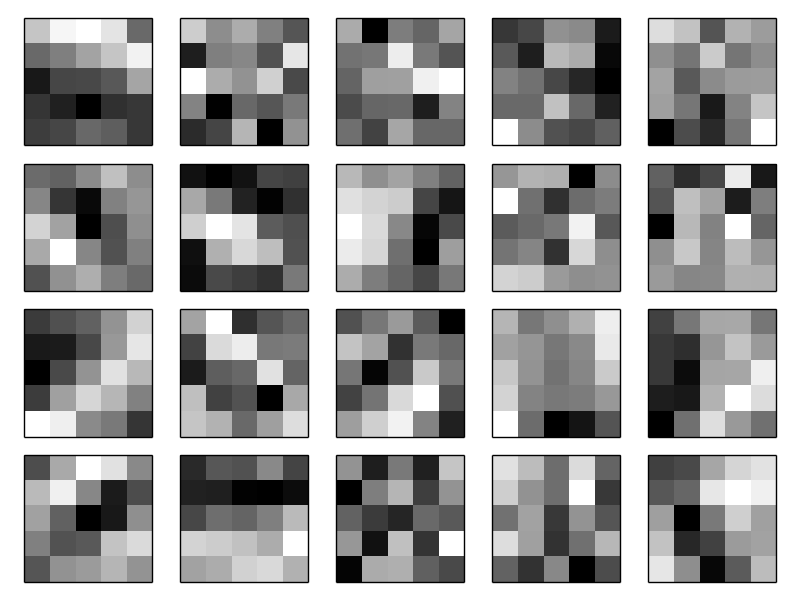
\includegraphics[width=.65\textwidth]{net_full_layer_0}
\end{center}

这 20 幅图像对应于 20 个不同的特征映射(或滤波器、核)。每个映射有一幅 $5 \times
5$ 块的图像表示,对应于\gls*{lrf}中的 $5 \times 5$ \gls*{weight}。白色块意味着一个小(典
  型的,更小的负数)\gls*{weight},所以这样的特征映射对相应的输入像素有更小的响应。更暗的
块意味着一个更大的\gls*{weight},所以这样的特征映射对相应的输入像素有更大的响应。非常粗略
地讲,上面的图像显示了卷积层作出响应的特征类型。

所以我们能从这些特征映射中得到什么结论?很明显这里有超出了我们期望的空间结构:这
些特征许多有清晰的亮和暗的子区域。这表示我们的网络实际上正在学习和空间结构相关的
东西。然而,除了那个,看清这些特征检测器在学什么是很困难的。当然,我们并不是在学
习(例如)\href{http://en.wikipedia.org/wiki/Gabor_filter}{Gabor 滤波器},它已经
被用在很多传统的图像识别方法中。实际上,现在有许多关于通过卷积网络来更好理解特征
的工作成果。如果你感兴趣,我建议从 Matthew Zeiler 和 Rob Fergus 的(2013)论文
\href{http://arxiv.org/abs/1311.2901}{Visualizing and Understanding
  Convolutional Networks} 开始。

\gls*{shared-weights}和\gls*{bias}的一个很大的优点是,它大大减少了参与的卷积网络的参数。
对于每个特征映射我们需要 $25 = 5 \times 5$ 个\gls*{shared-weights},加上一个共享
\gls*{bias}。所以每个特征映射需要 $26$ 个参数。如果我们有 $20$ 个特征映射,那么总共有
$20 \times 26 = 520$ 个参数来定义卷积层。作为对比,假设我们有一个全连接的第一层,
具有 $784 = 28 \times 28$ 个输入神经元,和一个相对适中的 $30$ 个隐藏神经元,正如
我们在本书之前的很多例子中使用的。总共有 $784 \times 30$ 个\gls*{weight},加上额外的 $30$
个\gls*{bias},共有 $23,550$个参数。换句话说,这个全连接的层有多达 $40$ 倍于卷积层的参
数。

当然,我们不能真正做一个参数数量之间的直接比较,因为这两个模型的本质是不同的径。
但是,直观地,使用卷积层的平移不变性似乎很可能减少全连接模型中达到同样性能的参数
数量。反过来,这将导致更快的卷积模型的训练,并最终,将有助于我们使用卷积层建立深
度网络。

顺便提一下,\textbf{卷积}(\textit{convolutional})这一名称源自方程~\eqref{eq:125}
中的操作符有时被称为一个\textbf{卷积}(\textit{convolution})。稍微更精确些,人
们有时把这个方程写成 $a^1 = \sigma(b + w * a^0)$,其中 $a^1$ 表示出自一个特征映
射的输出激活值集合,$a^0$ 是输入激活值的集合,而 $*$ 被称为一个卷积操作。我们不
打算深入使用卷积数学,所以你不用对此太担心。但是至少值得知道这个名称从何而来。\\

\textbf{\gls*{pooling}层:} 除了刚刚描述的卷积层,\gls*{cnn}也包含%
\textbf{\gls*{pooling}层}(\textit{pooling layers})。\gls*{pooling}层通常紧接着
在卷积层之后使用。它要做的是简化从卷积层输出的信息。

详细地说,一个\gls*{pooling}层取得从卷积层输出的每一个特征映射\footnote{这里使用
  的术语是不严格的。特别地,我用“特征映射”表示的意思不是通过卷积层计算出的函数,
  而是隐藏神经元从该层输出的激活值。这种术语的轻度滥用在研究文献中是相当普遍的。}并
且从它们准备一个凝缩的特征映射。例如,\gls*{pooling}层的每个单元可能概括了前一层
的一个(比如)$2 \times 2$ 的区域。作为一个具体的例子,一个常见的\gls*{pooling}
的程序被称为\textbf{最大值混合}(\textit{max-pooling})。在最大值\gls*{pooling}
中,一个\gls*{pooling}单元简单地输出其 $2 \times 2$ 输入区域的最大激活值,正如下
图说明的:
\begin{center}
  \includegraphics{tikz47}
\end{center}
注意既然从卷积层有 $24 \times 24$ 个神经元输出,\gls*{pooling}后我们得到 $12
\times 12$ 个神经元。

正如上面提到的,卷积层通常包含超过一个特征映射。我们将最大值\gls*{pooling}分别应
用于每一个特征映射。所以如果有三个特征映射,组合在一起的卷积层和最大值%
\gls*{pooling}层看起来像这样:
\begin{center}
  \includegraphics{tikz48}  
\end{center}

我们可以把最大值\gls*{pooling}看作一种网络询问是否有一个给定的特征在一个图像区域
中的哪个地方被发现的方式。然后它扔掉确切的位置信息。直观上,一旦一个特征被发现,
它的确切位置并不如它相对于其它特征的大概位置重要。一个很大的好处是,这样可以有很
多被更少地\gls*{pooling}的特征,所以这有助于减少在以后的层所需的参数的数目。

最大值\gls*{pooling}并不是用于\gls*{pooling}的仅有的技术。另一个常用的方法是
\textbf{L2 \gls*{pooling}}。这里我们取 $2 \times 2$ 区域中激活值的平方和的平方根,
而不是最大激活值。虽然细节不同,但其直观上和最大值\gls*{pooling}是相似的:L2
\gls*{pooling}是一种凝缩从卷积层输出的信息的方式。在实践中,两种技术都被广泛应用。
而且有时候人们使用其它\gls*{pooling}操作的类型。如果你正在尝试优化性能,你可以使
用验证数据来比较\gls*{pooling}的不同方法,并选择一个工作得最好的。但我们不打算惦
记这种细节上的优化。\\

\textbf{综合在一起:} 我们现在可以把这些思想都放在一起来构建一个完整的卷积神经网
络。它和我们刚看到的架构相似,但是有额外的一层 $10$ 个输出神经元,对应于 $10$ 个
可能的 MNIST 数字('0','1','2'等):
\begin{center}
  \includegraphics{tikz49}  
\end{center}

这个网络从 $28 \times 28$ 个输入神经元开始,这些神经元用于对 MNIST 图像的像素强
度进行编码。接着的是一个卷积层,使用一个 $5 \times 5$ \gls*{lrf}和 $3$ 个特征映
射。其结果是一个 $3 \times 24 \times 24$ 隐藏特征神经元层。下一步是一个最大值%
\gls*{pooling}层,应用于 $2 \times 2$ 区域,遍及 $3$ 个特征映射。结果是一个 $3
\times 12 \times 12$ 隐藏特征神经元层。

网络中最后连接的层是一个全连接层。更确切地说,这一层将最大值\gls*{pooling}层的%
\textbf{每一个}神经元连接到每一个输出神经元。这个全连接结构和我们之前章节中使用
的相同。然而,注意上面的图示,为了简化,我只使用了一个箭头,而不是显示所有的连接。
当然,你可以很容易想象到这些连接。

这个卷积架构和之前章节中使用的架构相当不同。但是总体的描述是相似的:一个由很多简
单的单元构成的网络,这些单元的行为由它们的\gls*{weight}和\gls*{bias}确定。而总体的目标仍然是一样
的:用训练数据来训练网络的\gls*{weight}和\gls*{bias},使得网络可以胜任分类输入数字。

特别的,正如本书中前面那样,我们将用\gls*{sgd}和\gls*{bp}训练我们的网络。这大部
分按照前面章节中完全相同的方式来处理。然而,我们确实需要对\gls*{bp}程序做些修改。
原因是我们之前的\hyperref[ch:HowThebackpropagationalgorithmworks]{\gls*{bp}的推
  导}是针对全连接层的网络。幸运的是,针对卷积和最大值\gls*{pooling}层的推导是简
单的。如果你想理解细节,那么我请你完成下面的问题。注意这个问题会花费些时间来完成,
除非你确实已经吸收了\hyperref[ch:HowThebackpropagationalgorithmworks]{前面的反向
  传播的推导}(这种情况下是容易的)。

\subsection*{问题}

\begin{itemize}
\item \textbf{卷积网络中的\gls*{bp}}\quad 在一个具有全连接层的网络中,\gls*{bp}
  的核心方程是 \eqref{eq:bp1}--\eqref{eq:bp4}(\hyperref[backpropsummary]{链接})。
  假设我们有这样一个网络,它包含有一个卷积层,一个最大值\gls*{pooling}层,和一个
  全连接的输出层,正如上面讨论的那样。\gls*{bp}的方程式要如何修改?
\end{itemize}

\section{卷积神经网络在实际中的应用}
\label{seq:convolutional_neural_networks_in_practice}

我们现在已经明白了\gls*{cnn}后面的核心思想。让我们通过实现一些卷积网络,并将它们
应用于 MNIST 数字分类问题,来看看它们如何在实践中工作。我们将使用的程序是
\lstinline!network3.py!,它是前面章节开发的 \lstinline!network.py! 和
\lstinline!network2.py! 的强化版本\footnote{注意 \lstinline!network3.py! 包含了
  源自 Theano 库文档中关于\gls*{cnn}(尤其是
    \href{http://deeplearning.net/tutorial/lenet.html}{LeNet-5} 的实现),Misha
  Denil 的\href{https://github.com/mdenil/dropout}{弃权的实现},以及
  \href{http://colah.github.io/}{Chris Olah} 的概念。}。如果你想跟着学,代码可以
从
\href{https://github.com/mnielsen/neural-networks-and-deep-learning/blob/master/src/network3.py}{GitHub}
上下载。注意我们将在下一节中解决 \lstinline!network3.py! 需要的代码。在这一节中,
我们将把 \lstinline!network3.py! 作为库来构建卷积网络。

程序 \lstinline!network.py! 和 \lstinline!network2.py! 是用 Python 和矩阵库Numpy
实现的。这些程序从最初的原理工作,并致力于\gls*{bp}、\gls*{sgd}等细节。但是现在
我们已经理解了这些细节,对于 \lstinline!network3.py! 我们打算使用一个称为
\href{http://deeplearning.net/software/theano/}{Theano} 的机器学习库\footnote{参
  见
  \href{http://www.iro.umontreal.ca/~lisa/pointeurs/theano_scipy2010.pdf}{Theano:
    A CPU and GPU Math Expression Compiler in Python},作者为 James Bergstra,
  Olivier Breuleux, Frederic Bastien, Pascal Lamblin, Ravzan Pascanu,
  Guillaume Desjardins, Joseph Turian, David Warde-Farley, 和 Yoshua Bengio
  (2010)。 Theano 也是流行的
  \href{http://deeplearning.net/software/pylearn2/}{Pylearn2} 和
  \href{http://keras.io/}{Keras} 神经网络库的基础。其它在本文写作时流行的神经网
  路库包括\href{http://caffe.berkeleyvision.org/}{Caffe} 和
  \href{http://torch.ch/}{Torch}。}。使用 Theano 使得实现针对\gls*{cnn}的%
\gls*{bp}很容易,因为它自动计算涉及到的映射。Theano 也比我们前面代码更快(那些代
  码是为了容易理解,不是为了运行速度),这使它可实际用于训练更复杂的网络。特别地,
Theano 的一个非常好的特性是它能够运行于 CPU 或者,如果可以,GPU 上。运行于 GPU上
可以提供显著的增速,而且,有助于实际用于更复杂的网络。

如果你想要跟着学,你需要可运行在你的系统上的 Theano。按照项目%
\href{http://deeplearning.net/software/theano/}{主页}上的说明来安装 Theano。接下
来的例子使用 Theano 0.6\footnote{当我发布这一章时,Theano 的当前版本变成了 0.7。
  我实际上已经在 Theano 0.7 版本中重新运行过这些例子并取得了和文中非常相似的结
  果。} 运行过。有些在没有 GPU 支持的 Mac OS X Yosemite 运行过。有些在有 NVIDIA
GPU 支持的 Ubuntu 14.04 中运行过。有些实验在两个系统中都运行过。为了让
\lstinline!networks3.py! 运行,你需要(适当地)把 \lstinline!networks3.py! 源码
中的 \lstinline!GPU! 标志设置为 \lstinline!True! 或者 \lstinline!False!。此外,
为了让 Theano 运行于 GPU 上,你可能会发现%
\href{http://deeplearning.net/software/theano/tutorial/using_gpu.html}{这份指导
  说明}有帮助。互联网上也有教程,很容易用 Google 搜索到,同样能帮助你让 Theano
工作。如果你手上的系统没有可用的 GPU,那么你可能想要看下
\href{http://aws.amazon.com/ec2/instance-types/}{Amazon Web Services} EC2 G2实例
类型。注意即使有 GPU 支持,代码仍然需要一些时间执行。许多实验要花费从几分钟到几
个小时的时间来运行。在 CPU 上可能需要花费数天时间来运行最复杂的实验。正如前面章
节里说的,我建议让程序运行着,同时继续阅读,偶尔回来检查下代码的输出。如果你用的
是 CPU,你可能需要对更复杂的实验减少训练\\gls*{epoch}的数量,或者整个忽略它们。

为了取得一个基线,我们将从一个浅层架构开始,它仅仅使用一个\gls*{hidden-layer},包含 $100$ 个
隐藏神经元。我们会训练 60 个\gls*{epoch},使用\gls*{learning-rate}为:$\eta =
0.1$,\gls*{mini-batch} 大小为 $10$,没有\gls*{regularization}。这样运
行\footnote{本节中的实验代码可以在%
  \href{https://github.com/mnielsen/neural-networks-and-deep-learning/blob/master/src/conv.py}{%
    这个脚本中}找到。注意,脚本中的代码只是简单地重复并相对于本节中的讨论。}:
\begin{lstlisting}[language=Python]
>>> import network3
>>> from network3 import Network
>>> from network3 import ConvPoolLayer, FullyConnectedLayer, SoftmaxLayer
>>> training_data, validation_data, test_data = network3.load_data_shared()
>>> mini_batch_size = 10
>>> net = Network([
        FullyConnectedLayer(n_in=784, n_out=100),
        SoftmaxLayer(n_in=100, n_out=10)], mini_batch_size)
>>> net.SGD(training_data, 60, mini_batch_size, 0.1, 
            validation_data, test_data)
\end{lstlisting}

我获得的一个最好的分类准确率是 $97.80$\%。这是 \lstinline!test_data! 上的分类准
确率,在这个取值的训练\gls*{epoch}的地方,我们在\lstinline!validation_data!上得到了
最好的分类准确率。使用验证数据来决定在何时对测试准确率估值有助于避免测试数据上的
\gls*{overfitting}(见前面关于验证数据使用的\hyperref[validation_explanation]{讨
    论})。我们将在下面遵循这个习惯。你的结构可能稍有不同,因为网络的\gls*{weight}和\gls*{bias}
是随机初始化的\footnote{实际上,在这个实验中我其实对这个架构的网络运行了三次独立
  的训练。然后我从这三次运行中报告了对应于最佳验证准确率的测试准确率。利用多次运
  行有助于减少结果中的变动,它在比较许多个架构时是很有用的,正如我们正在做的。除
  非明确指出,我在下面已经遵循了这个程序。在实践中,它对于所获得的结果不会带来什
  么区别。}。

这个 $97.80$\% 的准确率接近于\hyperref[chap3_98_04_percent]{第三章}中获得的
$98.04$\% 的准确率,使用一个相似的网络架构和学习超参数。特别地,两个例子都使用一
个浅层网络,具有单个包含有 $100$ 个隐藏神经元的\gls*{hidden-layer}。两者都训练 $60$ 个
\gls*{epoch},\gls*{mini-batch}大小为 $10$,\gls*{learning-rate} 为 $\eta = 0.1$。

然而,在之前的网络中有两个不同的地方。首先,我们%
\hyperref[sec:overfitting_and_regularization]{\gls*{regularization}}了之前的网络,
来帮助降低\gls*{overfitting}带来的影响。\gls*{regularization}当前的网络确实可以
提高准确率,但是得到的只是很小,所以我们将推迟到后面再来惦记%
\gls*{regularization}。第二,虽然之前的网络中的最终层使用了S型激活值和交叉熵代价
函数,当前网络使用一个\gls*{softmax}的最终层,以及对数似然代价函数。正如第三章中%
\hyperref[subsec:softmax]{解释}的,这不是一个大的改变。我没有为了任何特别深刻的
原因来做出这样的改变~——~主要是因为\gls*{softmax}和\gls*{log-likelihood}代价在现
代的图像分类网络中很常见。

我们能用一个更深的网络架构来做得比这些结果更好吗?

让我们从在网络开始位置的右边插入一个卷积层开始。我们将使用 $5 \times 5$ 局部感受
野,跨距为 $1$,$20$ 个特征映射。我们也会插入一个最大值\gls*{pooling}层,它用一
个 $2 \times 2$ 的\gls*{pooling}窗口来合并特征。所以总体的网络架构看起来很像上一
节讨论的架构,但是有一个额外的全连接层:
\begin{center}
  \includegraphics{simple_conv}  
\end{center}

在这个架构中,我们可以把卷积和\gls*{pooling}层看作是在学习输入训练图像中的%
\gls*{lrf},而后面的全连接层则在一个更抽象的层次学习,从整个图像整合全局信息。这
是一种常见的卷积神经网络模式。

让我们训练这样的一个网络,看看它表现怎样\footnote{这里我继续使用一个大小为 $10$
  的\gls*{mini-batch}。正如我们\hyperref[mini_batch_size]{前面讨论过的},使用更
  大的\gls*{mini-batch}可能提高训练速度。我继续使用相同的\gls*{mini-batch},主要
  是为了和前面章节中的实验保持一致。}:
\begin{lstlisting}[language=Python]
>>> net = Network([
        ConvPoolLayer(image_shape=(mini_batch_size, 1, 28, 28), 
                      filter_shape=(20, 1, 5, 5), 
                      poolsize=(2, 2)),
        FullyConnectedLayer(n_in=20*12*12, n_out=100),
        SoftmaxLayer(n_in=100, n_out=10)], mini_batch_size)
>>> net.SGD(training_data, 60, mini_batch_size, 0.1, 
            validation_data, test_data)
\end{lstlisting}

我们得到了 $98.78$\% 的准确率,这是相当大的改善,超过了我们以前结构的任何一个。
事实上,我们已经减少了超过三分之一的错误率,这是一个很大的进步。

在指定网络结构时,我把卷积和\gls*{pooling}层作为一个单一层对待。不管他们是被视为
分开的层还是作为一个单一的层在一定程度上是一个个人喜好的问题。
\lstinline!network3.py! 视他们为单个层,因为它使得 \lstinline!network3.py! 的代
码更紧凑。然而,如果需要的话,很容易修改 \lstinline!network3.py! 使得这些层可以
单独指定。

\subsection*{练习}

\begin{itemize}
\item 如果你删除了全连接层,只使用卷积--\gls*{pooling}层和\gls*{softmax}层,你得
  到了什么样的分类准确率?全连接层的加入有帮助吗?
\end{itemize}

我们能改进 $98.78$\% 的分类准确率吗?

让我们试着插入第二个卷积--\gls*{pooling}层。把它插在已有的卷积--\gls*{pooling}层
和全连接\gls*{hidden-layer}之间。我们再次使用一个 $5 \times 5$ \gls*{lrf},\gls*{pooling} $2
\times 2$ 的区域。让我们看看用前面相似的\gls*{hyper-params}训练会发生什么:
\begin{lstlisting}[language=Python]
>>> net = Network([
        ConvPoolLayer(image_shape=(mini_batch_size, 1, 28, 28), 
                      filter_shape=(20, 1, 5, 5), 
                      poolsize=(2, 2)),
        ConvPoolLayer(image_shape=(mini_batch_size, 20, 12, 12), 
                      filter_shape=(40, 20, 5, 5), 
                      poolsize=(2, 2)),
        FullyConnectedLayer(n_in=40*4*4, n_out=100),
        SoftmaxLayer(n_in=100, n_out=10)], mini_batch_size)
>>> net.SGD(training_data, 60, mini_batch_size, 0.1, 
            validation_data, test_data)        
\end{lstlisting}

再一次,我们得到了改善:现在我们达到了 $99.06$\% 的分类准确率。

在这里有两个很自然想到的问题。第一个问题是:应用第二个卷积--\gls*{pooling}层意味
着什么?实际上,你可以认为第二个卷积--\gls*{pooling}层输入 $12 \times 12$ 幅“图
像”,其“像素”代表原始输入图像中特定的局部特征的存在(或不存在)。所以你可以认
为这一层输入原始输入图像的一个版本。这个版本是经过抽象和凝缩过的,但是仍然有大量
的空间结构,所以使用第二个卷积--\gls*{pooling}层是有意义的。

这是一个令然满意的观点,但是引出了第二个问题。从前面层的输出涉及 $20$ 个独立的特
征映射,所以对第二个卷积--\gls*{pooling}层有 $20 \times 20 \times 12$ 个输入。就
好像我们有 $20$ 幅单独的图像输入给卷积--\gls*{pooling}层,而不是第一个卷
积--\gls*{pooling}层情况下的单幅图像。第二个卷积--\gls*{pooling}层里的神经元应该
如何响应这些多重的输入图像呢?实际上,我们将允许这一层中的每个神经元从它的%
\gls*{lrf}中的\textbf{所有} $20 \times 5 \times 5$ 输入神经元学习。更非正式的:
第二个卷积--\gls*{pooling}层中的特征检测器可访问\textbf{所有}前面层的特征,但仅
在其特定的\gls*{lrf}中\footnote{如果输入图像是有颜色的,这个问题会在第一层中出现。
  在这种情况下,对于每一个像素我们会有 3 个输入特征,对应于输入图像中的红色、绿
  色和蓝色通道。因此我们将允许特征检测器可访问所有颜色信息,但仅仅在一个给定的%
  \gls*{lrf}中。}。

\subsection*{问题}

\begin{itemize}
\item \textbf{使用\gls*{tanh}激活函数}\quad 在本书前面我已经几次提起过%
  \hyperref[subsec:other_models_of_artificial_neuron]{\gls*{tanh-func}}可以是一
  个比 \gls*{sigmoid-func}更好的激活函数。我们还没有实际采用过这些建议,因为我们
  已经用 S 型取得了大量进展。但现在让我们试试一些用\gls*{tanh}作为我们激活函数的
  实验。试着训练卷积和全连接层中具有\gls*{tanh}激活值的网络\footnote{注意你可以
    将 \lstinline!activation_fn=tanh! 作为一个参数传递给
    \lstinline!ConvPoolLayer! 和 \lstinline!FullyConnectedLayer! 类。}。开始时使
  用 S 型网络中使用的相同的超参数,但是训练 $20$ 个\gls*{epoch},而不是 $60$个。你
  的网络表现得怎么样?如果你继续训练到 $60$ 个\gls*{epoch}会怎样?试着将\gls*{tanh}
  和 S 型网络的每个\gls*{epoch}的验证准确率都绘制出来,都绘制到 $60$ 个\gls*{epoch}。如
  果你的结果和我的相似,你会发现\gls*{tanh}网络训练得稍微快些,但是最终的准确率
  非常相似。你能否解释为什么\gls*{tanh}网络可以训练得更快?你能否用 S型取得一个
  相似的训练速度,也许通过改变\gls*{learning-rate},或者做些调整\footnote{你也许可以
    回想 $\sigma(z) = (1+\tanh(z/2))/2$ 来找灵感。}?试着用五六个迭代学习超参数
  和网络架构,寻找\gls*{tanh}优于 S 型的方面。\textbf{注意:这是一个开放式问题。
    就我个人而言,我并没有找到太多切换为\gls*{tanh}的优势,虽然我没全面地做过实
    验,也许你会找到一个方法。无论如何,我们马上会发现切换到修正线性激活函数的一
    个优势,所以我们不会去深入使用\gls*{tanh}函数。}。
\end{itemize}

\textbf{使用\gls*{relu}:} 到现在为止,我们开发的网络实际上是一篇开创性的 1998论
文\footnote{\href{http://yann.lecun.com/exdb/publis/pdf/lecun-98.pdf}{"Gradient-based
    learning applied to document recognition"},作者为 Yann LeCun, Léon Bottou,
  Yoshua Bengio, 和 Patrick Haffner (1998)。细节上有很多不同,但大体上讲,我
  们的网络和论文中描述的网络非常相似。} 中使用的众多网络中一种的变化形式,这个网
络被称为 LeNet-5,并引入了 MNIST 问题。这为进一步实验并构筑理解和直观感受打下很
好的基础。特别是,有很多种我们可以改变网络来改善结果的方式。

作为开始,让我们改变我们的神经元,我们使用%
\hyperref[sec:other_models_of_artificial_neuron]{修正线性单元}而不是 S 型激活函
数。确切地说,我们将使用激活函数 $f(z) \equiv \max(0, z)$。我们将训练 $60$ 个%
\gls*{epoch},\gls*{learning-rate}为$\eta = 0.03$。我也发现用一些
\hyperref[sec:overfitting_and_regularization]{L2 \gls*{regularization}}也有点帮
助,使用\gls*{regularization}参数 $\lambda = 0.1$:
\begin{lstlisting}[language=Python]
>>> from network3 import ReLU
>>> net = Network([
        ConvPoolLayer(image_shape=(mini_batch_size, 1, 28, 28), 
                      filter_shape=(20, 1, 5, 5), 
                      poolsize=(2, 2), 
                      activation_fn=ReLU),
        ConvPoolLayer(image_shape=(mini_batch_size, 20, 12, 12), 
                      filter_shape=(40, 20, 5, 5), 
                      poolsize=(2, 2), 
                      activation_fn=ReLU),
        FullyConnectedLayer(n_in=40*4*4, n_out=100, activation_fn=ReLU),
        SoftmaxLayer(n_in=100, n_out=10)], mini_batch_size)
>>> net.SGD(training_data, 60, mini_batch_size, 0.03, 
            validation_data, test_data, lmbda=0.1)
\end{lstlisting}

我得到一个 99.23\% 的分类准确率。它稍微超过了 S 型的结果(99.06)。然而,在我所有
实验中我发现基于修正线性单元的网络,其性能始终优于基于 S 型激活函数的网络。似乎对
于这个问题切换到修正线性单元确实有收益。

是什么使得修正线性激活函数好于 S 型或者\gls*{tanh}函数?目前,我们对这个问题的答案有一
个很差的理解。实际上,修正线性单元只在过去几年才开始被广泛使用。最近才采用的原因
是以经验为依据的:一些人经常基于直觉或者启发式的理由试着用修正线性单
元\footnote{一个通常的理由是 $\max(0, z)$ 在 $z$ 取最大极限时不会饱和,不像 S 型
  神经元,而这有助于修正线性单元持续学习。到目前为止,这一辩解很好,但不是一个详
  细的理由,更多的是一个“就这样”的故事。注意我们在\hyperref[saturation]{第二章}里
  讨论过饱和的问题。}。他们在分类基准数据集时取得了很好的结果,并且其实践传播开了。
在一个理想的世界中,我们有一个理论告诉我们为什么样的应用选择什么样的激活函数。但
目前我们我们离这样的理想世界还有一条很长的路。如果通过选择一个更好的激活函数来取
得了进一步的重大改进,我一点也不会感到惊讶,我还期待在未来的几十年里,一个强大的
激活函数理论将被开发。今天,
我们仍然不得不依靠单凭经验的不足的理解。\\

\textbf{扩展训练数据:} 另一种我们可能希望改进结果的方法是以算法形式扩展训练数据。
扩展训练数据的一个简单的方法是将每个训练图像由一个像素来代替,无论是上一个像素,
一个像素,左边一个像素,或右边一个像素。我们可以通过在 shell 提示符中运行程
序 \lstinline!expand_mnist.py! 来这样做\footnote{\lstinline!expand_mnist.py! 的代
  码可以从%
  \href{https://github.com/mnielsen/neural-networks-and-deep-learning/blob/master/src/expand_mnist.py}{%
    这里}获取。}:
\begin{lstlisting}[language=Python]
$ python expand_mnist.py
\end{lstlisting}
 % move to separate file to avoid syntax error caused by '$' in EMACS.

运行这个程序取得 $50,000$ 幅 MNIST 训练图像并扩展为具有
$250,000$ 幅训练图像的训练集。然后我们可以使用这些训练图像来训练我们的网络。我们
将使用和上面一样的具有修正线性单元的网络。在我初始的实验中我减少了训练\gls*{epoch}的
数量~——~这讲得通,因为我们在训练 $5$ 倍的数据。但是实际上,扩展数据结果是相当多地
减少了\gls*{overfitting}的影响。所有,在做了一些实验后,我最终回到训练
$60$ 个\gls*{epoch}。不管怎样,让我们训练:
\begin{lstlisting}[language=Python]
>>> expanded_training_data, _, _ = network3.load_data_shared(
        "../data/mnist_expanded.pkl.gz")
>>> net = Network([
        ConvPoolLayer(image_shape=(mini_batch_size, 1, 28, 28), 
                      filter_shape=(20, 1, 5, 5), 
                      poolsize=(2, 2), 
                      activation_fn=ReLU),
        ConvPoolLayer(image_shape=(mini_batch_size, 20, 12, 12), 
                      filter_shape=(40, 20, 5, 5), 
                      poolsize=(2, 2), 
                      activation_fn=ReLU),
        FullyConnectedLayer(n_in=40*4*4, n_out=100, activation_fn=ReLU),
        SoftmaxLayer(n_in=100, n_out=10)], mini_batch_size)
>>> net.SGD(expanded_training_data, 60, mini_batch_size, 0.03, 
            validation_data, test_data, lmbda=0.1)
\end{lstlisting}

使用扩展后的训练数据我取得了一个 99.37\% 的训练准确率。所以这个几乎是微不足道的改变在分类准确率上给出了一个显著的改进。事实上,正如我们%
\hyperref[sec:other_techniques_for_regularization]{前面所讨论的},这种以算法形式
扩展数据的想法可以更进一步。提醒你一些早期讨论的结果:
在 2003 年,Simard,Steinkraus 和
Platt\footnote{\href{http://dx.doi.org/10.1109/ICDAR.2003.1227801}{Best
    Practices for Convolutional Neural Networks Applied to Visual Document
    Analysis},作者为 Patrice Simard, Dave Steinkraus, 和 John
  Platt (2003)。} 使用一个神经网络改进了他们的 MNIST 性能,达到了
$99.6$\%,这个网络以其它方式和我们的非常相似,使用两个卷积--\gls*{pooling}层,跟着一个具
有 $100$ 个神经元的隐藏的全连接层。在他们的架构中有一些细节上的不同~——~例如他们没
有利用修正线性单元~——~但是他们改进性能的关键是扩展训练数据。他们通过旋转,位移和
扭曲 MNIST 训练图像来扩展。他们还开发了一个“弹性扭曲”的流程,一种模拟当一个人写
字时手部肌肉随机振动的方式。通过组合所有这些流程,他们相当大地增加了训练数据的有
效规模,而这就是他们如何达到$99.6$\% 准确率的。

\subsection*{问题}

\begin{itemize}
\item 卷积层的想法是以一种横跨图像不变的方式作出反应。它看上去令人惊奇,然而,当
  我们做完所有输入数据的转换,网络能学习得更多。你能否解释为什么这实际上很合理?
\end{itemize}

\textbf{插入一个额外的全连接层:} 我们还能做得更好吗?一种可能性是使用和上面完全
相同的程序,但是扩展全连接层的规模。我试过 $300$ 和 $1,000$ 个神经元,分别取得
了 $99.46$\% 和 $99.43$\%。这很有趣,但对于前面的结果(99.37\%)并不是一个令人信
服的超越。

增加一个额外的全连接层怎样?让我们试着插入一个全连接层,这样我们就有两个 $100$ 个
隐藏神经元的全连接层:
\begin{lstlisting}[language=Python]
>>> net = Network([
        ConvPoolLayer(image_shape=(mini_batch_size, 1, 28, 28), 
                      filter_shape=(20, 1, 5, 5), 
                      poolsize=(2, 2), 
                      activation_fn=ReLU),
        ConvPoolLayer(image_shape=(mini_batch_size, 20, 12, 12), 
                      filter_shape=(40, 20, 5, 5), 
                      poolsize=(2, 2), 
                      activation_fn=ReLU),
        FullyConnectedLayer(n_in=40*4*4, n_out=100, activation_fn=ReLU),
        FullyConnectedLayer(n_in=100, n_out=100, activation_fn=ReLU),
        SoftmaxLayer(n_in=100, n_out=10)], mini_batch_size)
>>> net.SGD(expanded_training_data, 60, mini_batch_size, 0.03, 
            validation_data, test_data, lmbda=0.1)
\end{lstlisting}

这样做我取得一个 99.43\% 的测试准确率。再一次,扩展后的网络并没有帮助太多。运行
类似的试验,用包含$300$ 和 $1,000$ 个隐藏神经元的全连接层产生 $99.48$\% 和
$99.47$\% 的结果。这是令人鼓舞的,但仍然缺乏一个真正决定性的胜利。

\label{final_conv}
这里发生了什么事?扩展的,或者额外的全连接层真的对 MNIST 没帮助吗?或者说,我们
的网络有能力做得更好,但我们在用错误的方式学习?例如,也许我们可以用更强有力的规
范化技术来减小\gls*{overfitting}的趋势。一种可能性是第三章介绍的%
\hyperref[sec:other_techniques_for_regularization]{弃权}技术。回想弃权的基本思想
是在训练网络时随机地移除单独的激活值。这使得模型对单独依据的丢失更为强劲,因此不
太可能依赖于训练数据的特质。让我们试着应用弃权到最终的全连接层:
\begin{lstlisting}[language=Python]
>>> net = Network([
        ConvPoolLayer(image_shape=(mini_batch_size, 1, 28, 28), 
                      filter_shape=(20, 1, 5, 5), 
                      poolsize=(2, 2), 
                      activation_fn=ReLU),
        ConvPoolLayer(image_shape=(mini_batch_size, 20, 12, 12), 
                      filter_shape=(40, 20, 5, 5), 
                      poolsize=(2, 2), 
                      activation_fn=ReLU),
        FullyConnectedLayer(
            n_in=40*4*4, n_out=1000, activation_fn=ReLU, p_dropout=0.5),
        FullyConnectedLayer(
            n_in=1000, n_out=1000, activation_fn=ReLU, p_dropout=0.5),
        SoftmaxLayer(n_in=1000, n_out=10, p_dropout=0.5)], 
        mini_batch_size)
>>> net.SGD(expanded_training_data, 40, mini_batch_size, 0.03, 
            validation_data, test_data)
\end{lstlisting}

使用它,我们取得了 $99.60$\% 的准确率,这是一个显著的超越我们前面结果的进步,尤其
是我们主要的基准,具有 $100$ 个隐藏神经元的网络,其中我们达到了 $99.37$\%。

有两个值得注意的变化。

首先,我减少了训练\gls*{epoch}的数量到 $40$:弃权减少了\gls*{overfitting},所以我们学习得更
快。

其次,全连接\gls*{hidden-layer}有 $1,000$ 个神经元,不是之前使用的 $100$ 个。当然,在训练时弃
权有效地忽略了很多神经元。所以一些扩充是可以预期的。实际上,我试过
用 $300$ 和 $1,000$ 个隐藏神经元的实验,用 $1,000$ 个隐藏神经元(非常略微地)取得
了更好的验
证性能。\\

\textbf{使用一个组合的网络:} 一个简单的进一步提高性能的方法是创建几个神经网络,
然后让它们投票来决定最好的分类。例如,假设我们使用上述的方式训练了 $5$ 个不同的神
经网络,每个达到了接近于 $99.6$\% 的准确率。尽管网络都会有相似的准确率,他们很可
能因为不同的随机初始化产生不同的错误。在这 $5$ 个网络中进行一次投票来取得一个优于
单个网络的分类,似乎是合理的。

这听上去太好了,不像是真的,但是这种组合的方式是神经网络和其它机器学习技术都惯用
的伎俩。而它确实产生了更进一步的改善:我们最终得到了 99.67\% 的准确率。换句话说,
我们的网络组合正确分类了除了 $33$ 个之外所有的 $10,000$ 个测试图像。

剩余的测试集中的错误显示在下面。右上角的标签是按照 NMIST 数据的正确的分类,而右下
角的标签是我们组合网络的输出。
\begin{center}
  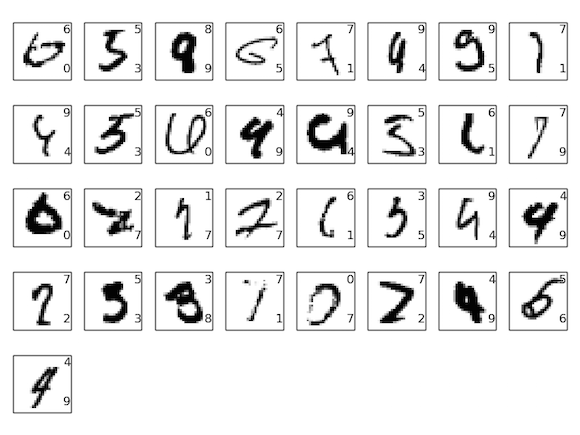
\includegraphics[width=.75\textwidth]{ensemble_errors}
\end{center}

值得去仔细看看这些。开头两个数字,一个 6 和一个 5,是我们的组合犯的真正的错误。然
而,它们也是可以理解的错误,人类也会犯。那个 6 确实看上去更像一个 0,而那个 5看上
去更像一个 3。第三幅图像,据称是一个 8,在我看来实际上更像一个 9。所以这里我站在
网络组合这边:我认为它比最初画出这些数字的人做得更好。另一方面,第四幅图像,那
个 6,确实看上去是我们网络分类错了。

如此等等。在大多数情况下我们网络的选择看上去至少是合理的,而在一些情况下我们比最
初写这些数字的人做得更好。总体而言,我们的网络提供卓越的性能,特别是当你认为它们
正确分类的 9,967 张图片,这是没有显示。在这种背景下,这里的不清晰的错误似乎是可以
理解的。甚至一个细心的人也会偶尔犯错误。因此我认为只有一个非常细心和有条理的人
才会做得更好。我们的网络正在接近人类的性能。\\

\textbf{为什么我们只对全连接层应用弃权:} 如果你仔细看上面的代码,你会注意到我们
只在网络的全链接部分应用了弃权,而不是卷积层。原则上我们可以在卷积层上应用一个类
似的程序。但是,实际上那没必要:卷积层有相当大的先天的对于\gls*{overfitting}的抵抗。原因是
\gls*{shared-weights}意味着卷积滤波器被强制从整个图像中学习。这使他们不太可能去选择在训练数据
中的局部特质。于是就很少有必要来应用其它\gls*{regularization},例如弃权。\\

\textbf{进一步:} 仍然有可能在 MNIST 上提高性能。Rodrigo Benenson 汇编了一份%
\href{http://rodrigob.github.io/are_we_there_yet/build/classification_datasets_results.html}{%
  信息汇总页面},显示这几年的进展,提供了论文的链接。这些论文许多使用深度卷积网络,
与我们已经使用的网络相似。如果你深入挖掘这些论文你会发现许多有趣的技术,并且你可
能乐于实现其中一些。如果你这样做,明智的做法是从一个简单的能被快速训练的网络开始
实现,这将有助于你更快地了解正在发生的事。

我不会概述这份近期成果的大部分内容。但是我忍不住有一个例外。它是一
篇 Cireșan、Meier、 Gambardella、 和 Schmidhuber 所著的 2010 年论
文\footnote{\href{http://arxiv.org/abs/1003.0358}{Deep, Big, Simple Neural Nets
    Excel on Handwritten Digit Recognition},作者为 Dan Claudiu Cireșan, Ueli
  Meier,Luca Maria Gambardella, 和 Jürgen Schmidhuber (2010)。}。我喜欢这篇
论文的地方是它是如此简单。其中的网络是一个许多层的神经网络,仅使用全连接层(没有
卷积层)。他们最成功的网络有分别包含
有 $2,500$,$2,000$,$1,500$,$1,000$ 和 $500$ 神经元的\gls*{hidden-layer}。他们使用和 Simard
等人类似的想法来扩展他们的训练数据。除了这些,他们没有使用其它的技巧,包括没有卷
积层:这是一个清晰的,简单的网络,这样的网络如果有足够的耐心,可以在 80 年代将其
训练(如果 MNIST 数据集已经有了),假设那时有足够的计算能力。他们达到了一
个99.65\% 的分类准确率,或多或少和我们一样。其关键是使用一个非常大,非常深的网络,
并且使用一块 GPU 来加速训练。这让他们训练了很多个\gls*{epoch}。他们也利用了他们的长
训练时间来逐渐地将\gls*{learning-rate}从 $10^{-3}$ 减小到 $10^{-6}$。试着用一个相似的
架构来匹配他们的结果是个很有趣的联系。\\

\textbf{为什么我们能够训练?} 我们在\hyperref[ch:WhyHardToTrain]{上一章}看到了深
的、多层的神经网络中的基本障碍。特别是,我们看到的梯度往往是相当不稳定的:当我们
从输出层移动到前面层,梯度趋于消失(消失的梯度问题)或爆炸(爆炸的梯度问题)。由
于梯度是我们用来训练的动机,这会导致问题。

我们如何避免这些结果?

当然,答案是我们没有回避这些结果。相反,我们已经做了一些事情,帮助我们继续进行。
特别地:(1)使用卷积层极大地减少了这些层中的参数的数目,使学习的问题更容易;(2)
使用更多强有力的\gls*{regularization}技术(尤其是弃权和卷积层)来减少\gls*{overfitting},否则它在更复杂的
网络中是更多的问题;(3)使用修正线性单元而不是 S 型神经元,来加速训练~——~依据经
验通常是 $3$--$5$ 倍;(4)使用 GPU 并愿意长时间的训练。特别是,在我们最后的实验
中,我们训练了 $40$ 个\gls*{epoch},使用一个 $5$ 倍于未经处理的 MNIST 训练数据的数据
集。在本书前面,我们主要用原始训练数据训练了 $30$ 个\gls*{epoch}。结合因素(3)和
(4),仿佛我们训练了比以前 $30$ 倍长的时间。

你的反应可能是:“就这样?这就是我们为了训练深度网络所要做的全部事情?为什么要小
题大做?”

当然,我们也已经使用了其它主意:利用充分大的数据集(为了避免\gls*{overfitting});使用正确
的代价函数(为了避免\hyperref[sec:the_cross-entropy_cost_function]{学习减速});
使用\hyperref[how_to_choose_a_neural_network's_hyper-parameters]{好的\gls*{weight}初始
  化}(也是为了避免因为神经元饱和引起的学习减速);%
\hyperref[sec:other_techniques_for_regularization]{以算法形式扩展训练数据}。我们
在前面章节中讨论了这些和其它想法,并在本章中的大部分已经可以重用这些想法了,而不
需要太多注解。

有了这样说法,这真的是一套相当简单的想法。在组合使用时简单,但功能强大。入门深度
学习变得非常容易!\\

\textbf{这些网络有多深?} 把卷积--\gls*{pooling}层算作一个层,我们最终的架构有 $4$ 个\gls*{hidden-layer}。
这样的一个真的应该被称为一个深度网络吗?当然,$4$ 个\gls*{hidden-layer}远远多于我们前面学习的
浅层网络。那些网络大部分只有一个\gls*{hidden-layer},或者偶尔有 $2$ 个\gls*{hidden-layer}。另一方面,2015年
使用最先进技术的深度网络有时候有几十个\gls*{hidden-layer}。我偶尔听到有人采取“更比你更深”的
态度,认为如果你没有跟上在隐层数目方面的攀比,那么你真的没有在做深度学习。我不赞
同这样的态度,部分因为它使得深度学习的定义像是时刻就有结果的事。深度学习中实际的
突破是认识到它超过浅的 $1$、$2$ 层的网络是切实可行的,这样的浅层网络直到 2000 年
中都占据优势。这确实是一个重大的突破,开启了更多有特殊意义的模型的探索。但除这之
外,层的数目并不是主要的基本利益关系。更确切地说,使用更深层的网络是一种用来帮助
实现其他目标工具~——~例如更好的分类精确率。
\\

\textbf{一些按部就班的话:} 在这一节中,我们从单个\gls*{hidden-layer}的浅层网络顺利转换到多层
卷积网络。这一切似乎很容易!我们做了一个改变,其中大部分,我们得到了改进。如果你
开始尝试,我可以保证事情不会总是那么顺利。原因是,我呈现的是一个清理过的叙述,省
略了许多实验~——~包括许多失败的实验。这个清理过的叙述,希望能帮助你清楚认识基本思
想。但它也有风险,传达着不完整的感觉。取得一个好的,可工作的网络会涉及到大量的试
验和错误,偶尔有挫折。在实践中,你应该预计会处理相当多的实验。为了加快这一进程,
你可能会发现回顾第三章关
于\hyperref[sec:how_to_choose_a_neural_network's_hyper-parameters]{如何选择一个神
  经网络的超参数}的讨论会有帮助,或许也看一些那一小节中的进一步阅读的建议。

\section{卷积网络的代码}
\label{sec:the_code_for_our_convolutional_networks}

好了,现在来看看我们的卷积网络代码,\lstinline!network3.py!。整体看来,程序结构类
似于 \lstinline!network2.py!,尽管细节有差异,因为我们使用了 Theano。首先我们来
看 \lstinline!FullyConnectedLayer! 类,这类似于我们之前讨论的那些神经网络层。下面
是代码

\begin{lstlisting}[language=Python]
class FullyConnectedLayer(object):

    def __init__(self, n_in, n_out, activation_fn=sigmoid, p_dropout=0.0):
        self.n_in = n_in
        self.n_out = n_out
        self.activation_fn = activation_fn
        self.p_dropout = p_dropout
        # Initialize weights and biases
        self.w = theano.shared(
            np.asarray(
                np.random.normal(
                    loc=0.0, scale=np.sqrt(1.0/n_out), size=(n_in, n_out)),
                dtype=theano.config.floatX),
            name='w', borrow=True)
        self.b = theano.shared(
            np.asarray(np.random.normal(loc=0.0, scale=1.0, size=(n_out,)),
                       dtype=theano.config.floatX),
            name='b', borrow=True)
        self.params = [self.w, self.b]

    def set_inpt(self, inpt, inpt_dropout, mini_batch_size):
        self.inpt = inpt.reshape((mini_batch_size, self.n_in))
        self.output = self.activation_fn(
            (1-self.p_dropout)*T.dot(self.inpt, self.w) + self.b)
        self.y_out = T.argmax(self.output, axis=1)
        self.inpt_dropout = dropout_layer(
            inpt_dropout.reshape((mini_batch_size, self.n_in)), self.p_dropout)
        self.output_dropout = self.activation_fn(
            T.dot(self.inpt_dropout, self.w) + self.b)

    def accuracy(self, y):
        "Return the accuracy for the mini-batch."
        return T.mean(T.eq(y, self.y_out))
\end{lstlisting}

\lstinline!__init__! 方法中的大部分都是可以自解释的,这里再给出一些解释。我们根据
正态分布随机初始化了\gls*{weight}和偏差。代码中对应这个操作的一行看起来可能很吓人,但其实
只在进行载入\gls*{weight}和偏差到 Theano 中所谓的共享变量中。这样可以确保这些变量可
在 GPU中进行处理。对此不做过深的解释。如果感兴趣,可以查
看 \href{http://deeplearning.net/software/theano/index.html}{Theano 的文档}。而这
种初始化的方式也是专门为 sigmoid 激活函数设计的(参
见\hyperref[sec:weight_initialization]{这里})。理想的情况是,我们初始化\gls*{weight}和偏
差时会根据不同的激活函数(如\gls*{tanh}和 Rectified Linear Function)进行调整。这个在
下面的问题中会进行讨论。初始方法 \lstinline!__init__! 以 
\lstinline!self.params = [self.W, self.b]! 结束。这样将该层所有需要学习的参数都归在一起。后
面,\lstinline!Network.SGD! 方法会使用 \lstinline!params! 属性来确定网络实例中什
么变量可以学习。

\lstinline!set_inpt! 方法用来设置该层的输入,并计算相应的输出。我使
用 \lstinline!inpt! 而非 \lstinline!input! 因为在python 中 \lstinline!input! 是一
个内置函数。如果将两者混淆,必然会导致不可预测的行为,对出现的问题也难以定位。注
意我们实际上用两种方式设置输入
的:\lstinline!self.input! 和 \lstinline!self.inpt_dropout!。因为训练时我们可能要
使用 dropout。如果使用 dropout,就需要设置对应丢弃的概
率 \lstinline!self.p_dropout!。这就是在 \lstinline!set_inpt! 方法的倒数第二
行 \lstinline!dropout_layer! 做的事。所
以 \lstinline!self.inpt_dropout! 和 \lstinline!self.output_dropout! 在训练过程中
使用,而 \lstinline!self.inpt! 和 \lstinline!self.output! 用作其他任务,比如衡量
验证集和测试集模型的准确度。

\lstinline!ConvPoolLayer! 和 \lstinline!SoftmaxLayer! 类定义和
\lstinline!FullyConnectedLayer! 定义差不多。所以我这儿不会给出代码。如果你感兴趣,
可以参考本节后面的 \lstinline!network3.py! 的代码。

尽管这样,我们还是指出一些重要的微弱的细节差别。明显一点的是,
在 \lstinline!ConvPoolLayer! 和 \lstinline!SoftmaxLayer! 中,我们采用了相应的合适
的计算输出激活值方式。幸运的是,Theano 提供了内置的操作让我们计算卷
积、max-pooling和 softmax 函数。

不大明显的,在我们引入\hyperref[sec:softmax]{softmax layer} 时,我们没有讨论如何
初始化\gls*{weight}和偏差。其他地方我们已经讨论过对 sigmoid 层,我们应当使用合适参数的正态
分布来初始化\gls*{weight}。但是这个启发式的论断是针对 sigmoid 神经元的(做一些调整可以用
于\gls*{tanh}神经元上)。但是,并没有特殊的原因说这个论断可以用在 softmax 层上。所以没
有一个先验的理由应用这样的初始化。与其使用之前的方法初始化,我这里会将所有权值和
偏差设置为 $0$。这是一个 ad hoc 的过程,但在实践使用过程中效果倒是很不错。

好了,我们已经看过了所有关于层的类。那么 Network 类是怎样的呢?让我们看
看 \lstinline!__init__! 方法:

\begin{lstlisting}[language=Python]
class Network(object):
    
    def __init__(self, layers, mini_batch_size):
        """Takes a list of `layers`, describing the network architecture, and
        a value for the `mini_batch_size` to be used during training
        by stochastic gradient descent.

        """
        self.layers = layers
        self.mini_batch_size = mini_batch_size
        self.params = [param for layer in self.layers for param in layer.params]
        self.x = T.matrix("x")  
        self.y = T.ivector("y")
        init_layer = self.layers[0]
        init_layer.set_inpt(self.x, self.x, self.mini_batch_size)
        for j in xrange(1, len(self.layers)):
            prev_layer, layer  = self.layers[j-1], self.layers[j]
            layer.set_inpt(
                prev_layer.output, prev_layer.output_dropout, self.mini_batch_size)
        self.output = self.layers[-1].output
        self.output_dropout = self.layers[-1].output_dropout
\end{lstlisting}

这段代码大部分是可以自解释的。\lstinline!self.params = [param for layer in ...]!
此行代码对每层的参数捆绑到一个列表中。\lstinline!Network.SGD! 方法会使
用 \lstinline!self.params! 来确定 \lstinline!Network! 中哪些变量需要学习。
而 \lstinline!self.x = T.matrix("x")! 和 \lstinline!self.y = T.ivector("y")! 则定
义了 Theano 符号变量 x 和 y。这些会用来表示输入和网络得到的输出。

这里不是 Theano 的教程,所以不会深度讨论这些变量指代什么东西。但是粗略的想法就是
这些代表了数学变量,而非显式的值。我们可以对这些变量做通常需要的操作:加减乘除,
作用函数等等。实际上,Theano 提供了很多对符号变量进行操作方法,如卷积、最大值\gls*{pooling}
等等。但是最重要的是能够进行快速符号微分运算,使用反向传播算法一种通用的形式。这
对于应用随机梯度下降在若干种网络结构的变体上特别有效。特别低,接下来几行代码定义
了网络的符号输出。我们通过下面这行

\begin{lstlisting}[language=Python]
init_layer.set_inpt(self.x, self.x, self.mini_batch_size)
\end{lstlisting}

设置初始层的输入。

请注意输入是以每次一个 mini-batch 的方式进行的,这就是\gls*{mini-batch}大小为何要指定
的原因。还需要注意的是,我们将输入 \lstinline!self.x! 传了两次:这是因为我们我们
可能会以两种方式(有dropout和无dropout)使用网络。\lstinline!for! 循环将符号变
量 \lstinline!self.x! 通过 \lstinline!Network! 的层进行前向传播。这样我们可以定义
最终的输出 \lstinline!output! 和 \lstinline!output_dropout! 属性,这些都
是 \lstinline!Network! 符号式输出。

现在我们理解了 \lstinline!Network! 是如何初始化了,让我们看看它如何使
用 \lstinline!SGD! 方法进行训练的。代码看起来很长,但是它的结构实际上相当简单。代
码后面也有一些注解。

\begin{lstlisting}[language=Python]
    def SGD(self, training_data, epochs, mini_batch_size, eta, 
            validation_data, test_data, lmbda=0.0):
        """Train the network using mini-batch stochastic gradient descent."""
        training_x, training_y = training_data
        validation_x, validation_y = validation_data
        test_x, test_y = test_data

        # compute number of minibatches for training, validation and testing
        num_training_batches = size(training_data)/mini_batch_size
        num_validation_batches = size(validation_data)/mini_batch_size
        num_test_batches = size(test_data)/mini_batch_size

        # define the (regularized) cost function, symbolic gradients, and updates
        l2_norm_squared = sum([(layer.w**2).sum() for layer in self.layers])
        cost = self.layers[-1].cost(self)+\
               0.5*lmbda*l2_norm_squared/num_training_batches
        grads = T.grad(cost, self.params)
        updates = [(param, param-eta*grad) 
                   for param, grad in zip(self.params, grads)]

        # define functions to train a mini-batch, and to compute the
        # accuracy in validation and test mini-batches.
        i = T.lscalar() # mini-batch index
        train_mb = theano.function(
            [i], cost, updates=updates,
            givens={
                self.x:
                training_x[i*self.mini_batch_size: (i+1)*self.mini_batch_size],
                self.y: 
                training_y[i*self.mini_batch_size: (i+1)*self.mini_batch_size]
            })
        validate_mb_accuracy = theano.function(
            [i], self.layers[-1].accuracy(self.y),
            givens={
                self.x: 
                validation_x[i*self.mini_batch_size: (i+1)*self.mini_batch_size],
                self.y: 
                validation_y[i*self.mini_batch_size: (i+1)*self.mini_batch_size]
            })
        test_mb_accuracy = theano.function(
            [i], self.layers[-1].accuracy(self.y),
            givens={
                self.x: 
                test_x[i*self.mini_batch_size: (i+1)*self.mini_batch_size],
                self.y: 
                test_y[i*self.mini_batch_size: (i+1)*self.mini_batch_size]
            })
        self.test_mb_predictions = theano.function(
            [i], self.layers[-1].y_out,
            givens={
                self.x: 
                test_x[i*self.mini_batch_size: (i+1)*self.mini_batch_size]
            })
        # Do the actual training
        best_validation_accuracy = 0.0
        for epoch in xrange(epochs):
            for minibatch_index in xrange(num_training_batches):
                iteration = num_training_batches*epoch+minibatch_index
                if iteration 
                    print("Training mini-batch number {0}".format(iteration))
                cost_ij = train_mb(minibatch_index)
                if (iteration+1) 
                    validation_accuracy = np.mean(
                        [validate_mb_accuracy(j) for j in xrange(num_validation_batches)])
                    print("Epoch {0}: validation accuracy {1:.2
                        epoch, validation_accuracy))
                    if validation_accuracy >= best_validation_accuracy:
                        print("This is the best validation accuracy to date.")
                        best_validation_accuracy = validation_accuracy
                        best_iteration = iteration
                        if test_data:
                            test_accuracy = np.mean(
                                [test_mb_accuracy(j) for j in xrange(num_test_batches)])
                            print('The corresponding test accuracy is {0:.2
                                test_accuracy))
        print("Finished training network.")
        print("Best validation accuracy of {0:.2
            best_validation_accuracy, best_iteration))
        print("Corresponding test accuracy of {0:.2
\end{lstlisting}

前面几行很直接,将数据集分解成 x 和 y 两部分,并计算在每个数据集中\gls*{mini-batch}的
数量。接下来的几行更加有意思,这也体现了 Theano 有趣的特性。那么我们就摘录详解一
下:

\begin{lstlisting}[language=Python]
  # define the (regularized) cost function, symbolic gradients, and updates
  l2_norm_squared = sum([(layer.w**2).sum() for layer in self.layers])
  cost = self.layers[-1].cost(self)+\
         0.5*lmbda*l2_norm_squared/num_training_batches
  grads = T.grad(cost, self.params)
  updates = [(param, param-eta*grad) 
             for param, grad in zip(self.params, grads)]
\end{lstlisting}

这几行,我们符号化地给出了\gls*{regularization}的对数似然代价函数,在梯度函数中计算了对应的导数,
以及对应参数的更新方式。Theano 让我们通过这短短几行就能够获得这些效果。唯一隐藏的
是计算 \lstinline!cost! 包含一个对输出层 \lstinline!cost! 方法的调用;该代码
在 \lstinline!network3.py! 中其他地方。但是,总之代码很短而且简单。有了所有这些定
义好的东西,下面就是定义 \lstinline!train_mini_batch! 函数,该 Theano 符号函数在
给定 minibatch 索引的情况下使用 \lstinline!updates! 来更新 \lstinline!Network! 的
参数。类似地,\lstinline!validate_mb_accuracy! 和 \lstinline!test_mb_accuracy! 计
算在任意给定的 minibatch 的验证集和测试集合上 \lstinline!Network! 的准确度。通过
对这些函数进行平均,我们可以计算整个验证集和测试数据集上的准确度。

\lstinline!SGD! 方法剩下的就是可以自解释的了~——~我们对次数进行迭代,重复使用训练
数据的\gls*{mini-batch}来训练网络,计算验证集和测试集上的准确度。

好了,我们已经理解了 \lstinline!network3.py! 代码中大多数的重要部分。让我们看看整
个程序,你不需过分仔细地读下这些代码,但是应该享受粗看的过程,并随时深入研究那些
激发出你好奇地代码段。理解代码的最好的方法就是通过修改代码,增加额外的特征或者重
新组织那些你认为能够更加简洁地完成的代码。代码后面,我们给出了一些对初学者的建议。
这儿是代码\footnote{在 GPU 上使用 Theano 可能会有点难度。特别地,很容易在从GPU 中
  拉取数据时出现错误,这可能会让运行变得相当慢。我已经试着避免出现这样的情况,但
  是也不能肯定在代码扩充后出现一些问题。对于你们遇到的问题或者给出的意见我洗耳恭
  听(mn@michaelnielsen.org)。}:

\lstinputlisting[language=Python]{code_samples/src/network3.py}

\subsection*{问题}

\begin{itemize}
\item 目前,\lstinline!SGD! 方法要求用户手动选择用于训练\gls*{epoch}的数量。前文中,
  我们讨论了一种自动选择训练次数的方法,也就是\hyperref[early_stopping]{提前停止}。
  修改 \lstinline!network3.py! 以实现提前停止。
\item 增加一个 \lstinline!Network! 方法来返回在任意数据集上的准确度。
\item 修改 \lstinline!SGD! 方法来允许学习率 $\eta$ 可以是训练次数的函数。\textbf{提
    示:在思考这个问题一段时间后,你可能会
    在\href{https://groups.google.com/forum/\#!topic/theano-users/NQ9NYLvleGc}{这
      个链接}找到有用的信息。}
\item 在本章前面我曾经描述过一种通过应用微小的旋转、扭曲和变化来扩展训练数据的方
  法。改变 \lstinline!network3.py! 来加入这些技术。\textbf{注意:除非你有充分多的内
    存,否则显式地产生整个扩展数据集是不大现实的。所以要考虑一些变通的方法。}
\item 在 \lstinline!network3.py! 中增加 \lstinline!load! 和 \lstinline!save! 方
  法。
\item 当前的代码缺点就是只有很少的用来诊断的工具。你能想出一些诊断方法告诉我们网
  络过匹配到什么程度么?加上这些方法。
\item 我们已经对\gls*{relu}及 S 型和\gls*{tanh-func}神经元使用了同样的初始方法。正
  如\hyperref[sec:weight_initialization]{这里所说},这种初始化方法只是适用
  于 \gls*{sigmoid-func}。假设我们使用一个全部使用 ReLU 的网络。试说明以常数 $c$ 倍调整网
  络的\gls*{weight}最终只会对输出有常数 $c$ 倍的影响。如果最后一层是 softmax,则会发生什么
  样的变化?对 ReLU 使用\gls*{sigmoid-func}的初始化方法会怎么样?有没有更好的初始化方
  法?\textbf{注意:这是一个开放的问题,并不是说有一个简单的自包含答案。还有,思考
    这个问题本身能够帮助你更好地理解包含 ReLU 的神经网络。}
\item 我们对于不稳定梯度问题
  的%
  \hyperref[sec:what_is_causing_the_vanishing_gradient_problem_unstable_gradients_in_deep_neural_nets]{%
    分析}实际上是针对 sigmoid 神经元的。如果是 ReLU,那分析又会有什么差异?你能够
  想出一种使得网络不太会受到不稳定梯度问题影响的好方法么?\textbf{注意:“好”这个
    词实际上就是一个研究性问题。实际上有很多容易想到的修改方法。但我现在还没有研
    究足够深入,能告诉你们什么是真正的好技术。}
\end{itemize}

\section{图像识别领域中的近期进展}
\label{sec:recent_progress_in_image_recognition}

在 1998 年,那年 MNIST 被初次提出,训练一个使用最先进技术的工作站,来达到明显差于
我们使用 GPU 并且训练少于一小时就能达到的准确率,要花费几周时间。因此,MNIST不再
是一个推动现有技术限制的问题;相反,训练的速度意味着它是个用于教授和学习目的的很
好的问题。与此同时,研究的重点已经转移,现代的工作涉及到更具挑战性的图像识别问题。
在这一节中,我简要介绍一些最近的使用神经网络的图像识别成果。

这一节和本书的大部分内容不同。贯穿本书我集中在可能引起持久兴趣的思想~——~如反向传
播、\gls*{regularization}、卷积网络。正如我写过的,我曾试图避免那些流行一时的成绩,但其长期价值
是未知的。在科学界,这样的成绩往往是生命短促的事物,它们逐渐消失,很少有持久的影
响。鉴于此,一个怀疑论者可能会说:“嗯,当真最近在图像识别中的进步是流行一时的例
子吗?在另外两年或三年中,一切会继续前进。所以当真这些成绩仅仅提起一些想要在绝对
前沿竞争的专家的兴趣?为什么要讨论呢?”

这样的一个怀疑论者是对的,最近论文的一些出色的细节,其被认为的重要性会逐渐减弱。
但过去几年已经看到了使用深度网络攻克极度困难的图像识别任务的非凡的进步。想象一下
一个科学历史学家在 2100 年写关于计算机视觉的东西。它们会把 2011 年至 2015 年(也
许超过几年)鉴定为由\gls*{cnn}驱动的取得重大突破的时间。那并不意味着深度卷积网
络在 2100 年仍然被使用,更不用提诸如弃权、修正线性单元等细节概念。但是它确实意味
着一个重要的变革正在发生,就现在,在知识的历史中。它有点像观察原子的发现,或者抗
生素的发明:具有历史意义的发明和探索。所以尽管我们不会深入挖掘细节,了解一些目
前正在进行的令人兴奋的探索是值得的。\\

\textbf{2012 LRMD 论文:} 让我从一篇源自斯坦福和谷歌的研究小组的 2012 年论
文\footnote{\href{http://research.google.com/pubs/pub38115.html}{Building
    high-level features using large scale unsupervised learning},作者为 Quoc
  Le,Marc'Aurelio Ranzato, Rajat Monga, Matthieu Devin, Kai Chen, Greg
  Corrado,Jeff Dean, 和 Andrew Ng (2012)。注意这篇论文中使用的网络架构在很多
  细节上和我们已经学习的深度卷积网络不同。然而,一般地说,LRMD 基于很多类似的思
  想。}开始。我把这篇论文称为 LRMD,取自前四位作者的姓。LRMD 使用一个神经网络来分
类 \href{http://www.image-net.org/}{ImageNet} 的图像,一个非常具有挑战性的图像识别
问题。他们使用的 2011 年 ImageNet 数据包含 16,000,000 幅全彩色图像,有 20,000个种
类。这些图像收集自开放的网络,由亚马逊的 Mechanical Turk 服务部门的员工分类。这里
有一些 ImageNet 图像\footnote{这些取自 2014 年的数据集,其相比 2011 年的有点改变。
  然而在质的方面,这个数据集是非常相似的。关于 ImageNet 的详情可以在原始
  的 ImageNet 论文 \href{http://www.image-net.org/papers/imagenet_cvpr09.pdf}{
    ImageNet: a large-scale hierarchical image database} 中找到,作者为 Jia
  Deng,Wei Dong,Richard Socher, Li-Jia Li, Kai Li, 和 Li
  Fei-Fei (2009)。}:

\begin{center}
  
\includegraphics[height=80pt]{imagenet1.jpg}%
  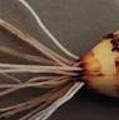
\includegraphics[height=80pt]{imagenet2.jpg}%
  
\includegraphics[height=80pt]{imagenet3.jpg}%
  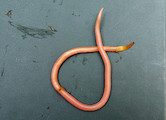
\includegraphics[height=80pt]{imagenet4.jpg}
\end{center}

这些是各自分类中的圆线刨、褐根腐菌、煮过的牛奶和常见的蛔虫。如果你正在找个挑战,
我鼓励你去访
问 ImageNet 的\href{http://www.image-net.org/synset?wnid=n03489162}{手工具}列表,
这个列表把圆线刨、短刨、倒角刨和大概一打的其它刨子类型从其它种类中区分开。我不知
道你怎么样,但是我是没有信心区分所有这些工具的类型。这明显是一个比 MNIST 更有挑战
性的图像识别任务。LRMD 的网络获得了一个不错的 15.8\% 的准确率来正确分类 ImageNet
图像。那听上去可能不算令人印象深刻,但是和以前的最好成绩 9.3\% 准确率相比已经是巨
大的进步了。这个跳跃暗示着神经网络也许能提供一个强大的方法来应对非常有挑战性的图
像识别任务,比如 ImageNet。\\

\textbf{2012 KSH 论文:} LRMD 的成果被一篇 Krizhevsky,
Sutskever 和 Hinton (KSH)
\footnote{\href{http://www.cs.toronto.edu/~fritz/absps/imagenet.pdf}{ImageNet
    classification with deep convolutional neural networks},作者为 Alex
  Krizhevsky,Ilya Sutskever, 和 Geoffrey E. Hinton (2012)。} 的 2012 年论文追
随。KSH 训练和测试一个深度\gls*{cnn},它使用 ImageNet数据的一个有限的子集。他们
使用的子集来自一个流行的机器学习竞赛~——~ImageNet Large-Scale Visual Recognition
Challenge(ILSVRC)。使用一个竞赛用的数据集给了他们一个很好的和其它领先技术比较的
途径。ILSVRC-2012 训练集包含有大约 1,200,000 幅 ImageNet 图像,取自 1,000 个种类。
验证和测试集分别包含有 50,000 和 150,000 幅图像,各自取自同样的1,000 个种类。

运行 ILSVRC 竞赛一个困难的地方是很多 ImageNet 图像包含了多个物体。假设一幅显示一
条拉布拉多犬追逐一个足球的图像。这幅图像所谓“正确的” ImageNet 分类也许是一条拉
布拉多犬。如果一个算法把这个图像标记为一个足球,它应该被扣分吗?由于这种歧义性,
如果实际的 ImageNet 分类在一个算法认为最有可能的 $5$ 个分类中,那么这个算法就被认
为是正确的。通过这个前 $5$ 标准,KSH 的深度卷积网络达到了一个 $84.7$\% 的准确率,
大大好于次优的参赛者,后者取得了 $73.8$\% 的准确率。使用更严格的必需准确标记的标
准,KSH 的网络达到了 $63.3$\% 的准确率。

既然 KSH 网络激励了随后的成果,值得对它简要描述一下。正如我们看到的,尽管要更精细,
它非常接近于这一章中我们之前训练的网络。KSH 使用一个深度\gls*{cnn},在两
个 GPU上训练。他们使用两块 GPU 是因为当时使用的特定的 GPU 型号(一块 NVIDIA
GeForce GTX 580)没有足够的片上存储器来保存整个网络。所以他们用两块 GPU 把网络分
成两个部分。

KSH 网络有 $7$ 个隐藏神经元层。前 $5$ 个\gls*{hidden-layer}是卷积层(有些具有最大值\gls*{pooling}),而
接下来的 $2$ 层是全连接层。输出层是一个 $1,000$ 个单元的柔性最大值层,对应于
那$1,000$ 个图像类别。这是这个网络的一个草图,取自 KSH 论文\footnote{感谢 Ilya
  Sutskever。}。细节在下面讨论。注意许多层被分成 $2$ 个部分,对应于 $2$ 块 GPU。
\begin{center}
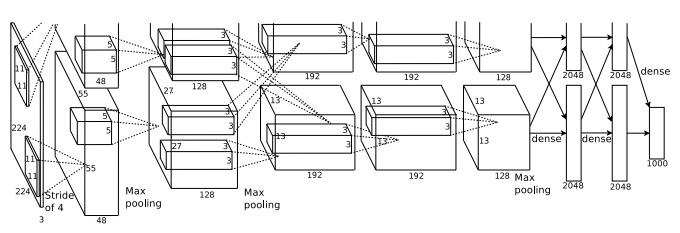
\includegraphics[width=.9\textwidth]{KSH}
\end{center}

输入层包含 $3 \times 224 \times 224$ 个神经元,对应于一幅 $224 \times 224$ 图像
的 RBG 值。回想前面提到的,ImageNet 包含有不同分辨率的图像。这引起了一个问题,因
为一个神经网络的输入层通常是固定大小。KSH 通过缩放每幅图像使得长和宽中短的长度
为 $256$ 来处理。然后他们从缩放后的图像中裁剪出一个 $256 \times 256$ 的区域。最
后,KSH 从 $256 \times 256$ 的图像中随机提取出 $224 \times 224$ 的子图像(和水平
反射)。他们把这个随机的裁剪用作扩展训练数据的方式,这样减少\gls*{overfitting}。这在一个例
如 KSH 的大的网络中尤其有帮助。正是这些 $224 \times 224$ 图像被用于网络的输入。在
大多数情况下裁剪后的图像仍然包含有未改动图像的主要物体。

这是 KSH 论文中许多核心思想一个总体概况。我已经忽略了一些细节,对此你可以看下论文。
你也可以看下 Alex
Krizhevsky 的\href{https://code.google.com/p/cuda-convnet/}{cuda-convnet}(和接替
版本),它包含有实现这许多思想的代码。一个基于 Theano 的实
现\footnote{\href{http://arxiv.org/abs/1412.2302}{Theano-based large-scale
    visual recognition with multiple GPUs},作者为 Weiguang Ding, Ruoyan
  Wang,Fei Mao, 和 Graham Taylor (2014)。},代码可以在%
\href{https://github.com/uoguelph-mlrg/theano_alexnet}{这里}得到。尽管使用
多 GPU会让情况变得复杂,但代码本身还是类似于这章我们写出来的那些。Caffe 神经网络
框架也包含一个 KSH 网络的版本,详细参见
\href{http://caffe.berkeleyvision.org/model_zoo.html}{Model Zoo}。\\

\textbf{2014 ILSVRC 竞赛:} 自 2012 年以来,研究一直在快速推进。看
看 2014 年的ILSVRC 竞赛。和 2012 一样,这次也包括了一个 $120,000$ 张图
像,$1,000$ 种类别,而优值系数是前 $5$ 个预测是否包含正确的分类。获胜团队,主要来
自谷歌\footnote{\href{http://arxiv.org/abs/1409.4842}{Going deeper with
    convolutions},作者为 Christian Szegedy, Wei Liu, Yangqing Jia, Pierre
  Sermanet,Scott Reed, Dragomir Anguelov, Dumitru Erhan, Vincent Vanhoucke,
  和 Andrew Rabinovich (2014)。},使用了包含 $22$ 层神经元的深度卷积网络。他们
称此为 GoogLeNet,作为向 LeNet-5 的致敬。GoogLeNet 达到了 93.33\% 的前 $5$ 准确率,
远超 2013 年的获胜者(\href{http://www.clarifai.com/}{Clarifai},88.3\%)和2012
年的获胜者(KSH,84.7\%)。

那么 GoogLeNet 93.33\% 的准确率又是多好呢?在 2014 年,一个研究团队写了一篇关
于ILSVRC 竞赛的综述文章\footnote{\href{http://arxiv.org/abs/1409.0575}{ImageNet
    large scale visual recognition challenge},作者为 Olga Russakovsky, Jia
  Deng,Hao Su, Jonathan Krause, Sanjeev Satheesh, Sean Ma, Zhiheng
  Huang,Andrej Karpathy, Aditya Khosla, Michael Bernstein, Alexander C.
  Berg, 和Li Fei-Fei(2014)。}。其中有个问题是人类在这个竞赛中能表现得如何。为
了做这件事,他们构建了一个系统让人类对 ILSVRC 图像进行分类。其作者之一 Andrej
Karpathy 在一篇%
\href{http://karpathy.github.io/2014/09/02/what-i-learned-from-competing-against-a-convnet-on-imagenet/}{%
  博文}中解释道,让人类达到 GoogLeNet 的性能确实很困难:

\begin{quote}
  ...从 1000 个类别中挑选出 5 个来标记图像的任务很快被证明是非常具有挑战性的,甚
  至对一些已经在 ILSVRC 和它同级别上工作一段时间的实验室里的朋友也是如此。开始我
  们以为能把它放在[Amazon Mechanical Turk]上。然后我们想过付费招募些还未毕业的
  大学生。然后我组织了一个只有实验室里有强烈标记热情的人(专家级标记人员)参与的
  标记聚会。然后我开发了一个修改了接口的 GoogLeNet 预测来把多余的类别数量从 1000
  减少到只有 100。它仍然太困难了~——~大家仍然持续地错过正确的类别并达到
  了 13--15\% 的错误率。最后我意识到为了有竞争力地接近 GoogLeNet,最有效率的做法
  是坐下来亲自完成痛苦的长期训练过程以及随后仔细的注记... 标记以每分钟 1 个的速度
  完成,但随着时间的推移减少了... 有些图像容易识别,同时有些图像(诸如那些有细密
  纹理的狗,鸟,或者猴子的品种)会需要几倍的集中精力。我变得非常擅长鉴别狗的品
  种... 基于我致力于的图像样本,GoogLeNet 分类的误差结果为 6.8\%... 我自己的误差
  最终为 5.1\%,大约以 1.7\% 的差距胜过。
\end{quote}

换言之,一个专家级别的人类,非常细心地检查图像,付出很大的努力才能够微弱胜过深度
神经网络。实际上,Karpathy 指出第二个人类专家,用小点的图像样本训练后,只能达
到 12.0\% 的 top-5 错误率,明显弱于 GoogLeNet。大概有一半的错误都是专家“难以发现
和认定正确的类别究竟是什么”。

这些都是令人惊奇的结果。确实,在这项成果后,很多团队也报告 top-5 错误率实际
上\textbf{好}过 5.1\%。这有时候在媒体上被报道成系统有超过人类的视觉。尽管这些结构是
很振奋人心的,但是这样的报道只能算是一种误解,认为系统在视觉上超过了人类,事实上
并非这样。ILSVRC 竞赛问题在很多方面都是受限的~——~在公开的网络上获得图像并不具备在
实际应用中的代表性!而且 top-5 标准也是非常人工设定的。我们在图像识别,或者更宽泛
地说,计算机视觉方面的研究,还有很长的路要走。当然看到近些年的这么多进展,还是很
鼓舞人心的。\\

\textbf{其它活动:} 上面关注于 ImageNet,但是也还有一些其他的使用神经网络进行图像
识别的工作。我们也介绍一些进展。

一个鼓舞人心的应用上的结果就是 Google 的一个团队做出来的,他们应用深度卷积网络在
识别 Google 的街景图像库中街景数字
上\footnote{\href{http://arxiv.org/abs/1312.6082}{Multi-digit Number Recognition
    from Street View Imagery using Deep Convolutional Neural Networks},作者
  为 Ian J. Goodfellow, Yaroslav Bulatov, Julian Ibarz, Sacha
  Arnoud, 和 Vinay Shet(2013)。}。在他们的论文中,对接近 $100,000,000$ 街景数
字的自动检测和自动转述已经能打到与人类不相上下的程度。系统速度很快:在一个小时内
将法国所有的街景数字都转述了。他们说道:“拥有这种新数据集能够显著提高 Google
Maps 在一些国家的地理精准度,尤其是那些缺少地理编码的地区。”他们还做了一个更一般
的论断:“我们坚信这个模型,已经解决了很多应用中字符短序列的 OCR 问题。 ”

我可能已经留下了印象——所有的结果都是令人兴奋的正面结果。当然,目前一些有趣的研究
工作也报道了一些我们还没能够真的理解的根本性的问题。例如,2013 年一篇论
文\footnote{\href{http://arxiv.org/abs/1312.6199}{Intriguing properties of
    neural networks},作者为 Christian Szegedy,Wojciech Zaremba, Ilya
  Sutskever, Joan Bruna, Dumitru Erhan, Ian Goodfellow,和 Rob
  Fergus (2013)}指出,深度网络可能会受到有效盲点的影响。看看下面的图示。左侧是
被网络正确分类的 ImageNet 图像。右边是一幅稍受干扰的图像(使用中间的噪声进行干扰)
结果就没有能够正确分类。作者发现对每幅图片都存在这样的“对手”图像,而非少量的特
例。

\begin{center}
  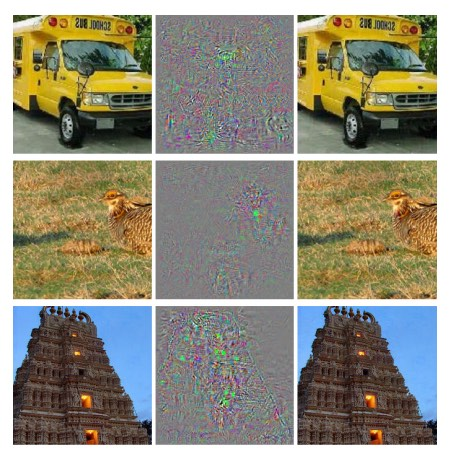
\includegraphics[width=.75\textwidth]{adversarial.jpg}
\end{center}

这是一个令人不安的结果。论文使用了基于同样的被广泛研究使用的 KSH 代码。尽管这样的
神经网络计算的函数在理论上都是连续的,结果表明在实际应用中,可能会碰到很多非常不
连续的函数。更糟糕的是,他们将会以背离我们直觉的方式变得不连续。真是烦心啊。另外,
现在对这种不连续性出现的原因还没有搞清楚:是跟损失函数有关么?或者激活函数?又或
是网络的架构?还是其他?我们一无所知。

现在,这些问题也没有听起来这么吓人。尽管对手图像会出现,但是在实际场景中也不常见。
正如论文指出的那样:

\begin{quote}
  对手反例的存在看起来和网络能获得良好的泛化性能相违背。实际上,如果网络可以很好
  地泛化,会受到这些难以区分出来的对手反例怎么样的影响?解释是,对手反例集以特别
  低的概率出现,因此在测试集中几乎难以发现,然而对手反例又是密集的(有点像有理数
  那样),所以会在每个测试样本附近上出现。
\end{quote}

我们对神经网络的理解还是太少了,这让人觉得很沮丧,上面的结果仅仅是近期的研究成果。
当然了,这样结果带来一个主要好处就是,催生出一系列的研究工作。例如,最近一篇文
章\footnote{\href{http://arxiv.org/abs/1412.1897}{Deep Neural Networks are
    Easily Fooled: High Confidence Predictions for Unrecognizable Images},作者
  为 Anh Nguyen, Jason Yosinski, 和 Jeff Clune(2014)。} 说明,给定一个训练好
的神经网络,可以产生对人类来说是白噪声的图像,但是网络能够将其确信地分类为某一类。
这也是我们需要追寻的理解神经网络和图像识别应用上的研究方向。

虽然遇到这么多的困难,前途倒还是光明的。我们看到了在众多相当困难的基准任务上快速
的研究进展。同样还有实际问题的研究进展,例如前面提到的街景数字的识别。但是需要注
意的是,仅仅看到在那些基准任务,乃至实际应用的进展,是不够的。因为还有很多根本性
的现象,我们对其了解甚少,就像对手图像的存在问题。当这样根本性的问题还亟待发现
(或者解决)时,盲目地说我们已经接近最终图像识别问题的答案就很不合适了。这样的根
本问题当然也会催生出不断的后续研究。

\section{其他的深度学习模型}
\label{sec:other_approaches_to_deep_neural_nets}

在整本书中,我们聚焦在解决 MNIST 数字分类问题上。这一“下金蛋的”问题让我们深入理
解了一些强大的想法:随机梯度下降,反向传播,卷积网络,正规化等等。但是该问题却也是相当
狭窄的。如果你研读过神经网络的研究论文,那么会遇到很多这本书中未曾讨论的想
法:RNN,Boltzmann Machine,生成式模型,迁移学习,强化学习等等……等等!(太多了)
神经网络是一个广阔的领域。然而,很多重要的想法都是我们书中探讨过的那些想法的变种,
在有了本书的知识基础上,可能需要一些额外的努力,便可以理解这些新的想法了。所以在
本节,我们给出这些想法的一些介绍。介绍本身不会非常细节化,可能也不会很深入——倘若
要达成这两点,这本书就得扩展相当多内容了。因此,我们接下来的讨论是偏重思想性的启
发,尝试去激发这个领域的产生丰富的概念,并将一些丰富的想法关联于前面已经介绍过的
概念。我也会提供一些其他学习资源的连接。当然,链接给出的很多想法也会很快被超过,
所以推荐你学会搜索最新的研究成果。尽管这样,我还是很期待众多本质的想法能够受到足
够久的关注。\\

\textbf{\gls*{rnn}(RNNs):} 在前馈神经网络中,单独的输入完全确定了剩下的层上的
神经元的激活值。可以想象,这是一幅静态的图景:网络中的所有事物都被固定了,处于一
种“冰冻结晶”的状态。但假如,我们允许网络中的元素能够以动态方式不断地比那话。例
如,隐藏神经元的行为不是完全由前一层的隐藏神经元,而是同样受制于更早的层上的神经
元的激活值。这样肯定会带来跟前馈神经网络不同的效果。也可能隐藏和输出层的神经元的
激活值不会单单由当前的网络输入决定,而且包含了前面的输入的影响。

拥有这类时间相关行为特性的神经网络就是\textbf{\gls{rnn}},常写作 \textbf{RNN(s)}。
当然有不同的方式来从数学上给出 RNN 的形式定义。你可以参考
\href{http://en.wikipedia.org/wiki/Recurrent_neural_network}{维基百科上的 RNN 介
  绍}来看看 RNN。在我写作本书的时候,维基百科上介绍了超过 13 种不同的模型。但除
了数学细节,更加一般的想法是,RNN 是某种体现出了随时间动态变化的特性的神经网络。
也毫不奇怪,RNN 在处理时序数据和过程上效果特别不错。这样的数据和过程正是语音识别
和自然语言处理中常见的研究对象。

RNN 被用来将传统的算法思想,比如说 Turing 机或者编程语言,和神经网络进行联系上。%
\href{http://arxiv.org/abs/1410.4615}{这篇 2014 年的论文}提出了一种 RNN 可以以
python 程序的字符级表达作为输入,用这个表达来预测输出。简单说,网络通过学习来理
解某些 python 的程序。\href{http://arxiv.org/abs/1410.5401}{第二篇论文}同样是
2014 年的,使用 RNN 来设计一种称之为 “神经 Turing 机” 的模型。这是一种通用机器
整个结构可以使用梯度下降来训练。作者训练 NTM 来推断对一些简单问题的算法,比如说
排序和复制。

不过正如在文中提到的,这些例子都是极其简单的模型。学会执行
\lstinline!print(398345+42598)!  并不能让网络称为一个正常的 Python 解释器!对于
这些想法,我们能推进得多远也是未知的。结果都充满了好奇。历史上,神经网络已经在传
统算法上失败的模式识别问题上取得了一些成功。另外,传统的算法也在神经网络并不擅长
的领域里占据上风。今天没有人会使用神经网络来实现 Web 服务器或者数据库程序。研究
出将神经网络和传统的算法结合的模型一定是非常棒的。RNN 和 RNN 给出的启发可能会给
我们不少帮助。RNN 同样也在其他问题的解决中发挥着作用。在语音识别中,RNN 是特别有
效的。例如,基于 RNN 的方法,已经在音位识别中取得了准确度的领先。同样在开发人类
语言的上改进模型中得到应用。更好的语言模型意味着能够区分出发音相同的那些词。例如,
好的语言模型,可以告诉我们“to infinity and beyond”比“two infinity and
beyond”更可能出现,尽管两者的发音是相同的。RNN 在某些语言的标准测试集上刷新了记
录。

在语音识别中的这项研究其实是包含于更宽泛的不仅仅是 RNN 而是所有类型的深度神经网
络的应用的一部分。例如,基于神经网络的方法在大规模词汇的连续语音识别中获得极佳的
结果。另外,一个基于深度网络的系统已经用在了 Google 的 Android 操作系统中(详见
  \href{http://research.google.com/pubs/VincentVanhoucke.html}{Vincent Vanhoucke
    的 2012-2015 论文})。

我刚刚讲完了 RNN 能做的一小部分,但还未提及他们如何工作。可能你并不诧异在前馈神
经网络中的很多想法同样可以用在 RNN 中。尤其是,我们可以使用梯度下降和\gls*{bp}的
直接的修改来训练 RNN。还有其他一些在前馈神经网络中的想法,如正规化技术,卷积和代
价函数等都在 RNN 中非常有效。还有我们在书中讲到的很多技术都可以适配一下RNN 场景。\\

\textbf{\gls{lstm}(LSTMs):} 影响 RNNs 的一个挑战是前期的模型会很难训练,甚至
比前馈神经网络更难。原因就是我们在\hyperref[ch:WhyHardToTrain]{上一章}提到的不稳
定梯度的问题。回想一下,这个问题的通常表现就是在反向传播的时候梯度越变越小。这就
使得前期的层学习非常缓慢。在 RNN 中这个问题更加糟糕,因为梯度不仅仅通过层反向传
播,还会根据时间进行反向传播。如果网络运行了一段很长的时间,就会使得梯度特别不稳
定,学不到东西。幸运的是,可以引入一个称为长短期记忆(long short-term memory)的
单元进入 RNN 中。LSTM 最早是由
\href{http://dx.doi.org/10.1162/neco.1997.9.8.1735}{Hochreiter 和 Schmidhuber在
  1997 年提出},就是为了解决这个不稳定梯度的问题。LSTM 让 RNN 训练变得相当简单,
很多近期的论文(包括我在上面给出的那些)都是用了 LSTM 或者相关的想法。\\

\textbf{深度信念网络,生成式模型和玻尔兹曼机:} 对深度学习的兴趣产生于 2006 年,
最早的论文就是解释如何训练称为\textbf{\gls{dbn}}(DBN)的神经网络\footnote{参见
  Geoffrey Hinton, Simon Osindero 和 Yee-Whye Teh 在 2006 年的
  \href{http://www.cs.toronto.edu/~hinton/absps/fastnc.pdf}{A fast learning
    algorithm for deep belief nets}, 及 Geoffrey Hinton 和 Ruslan Salakhutdinov
  在 2006 年的相关工作
  \href{http://www.sciencemag.org/content/313/5786/504.short}{Reducing the
    dimensionality of data with neural networks}}。DBN 在之后一段时间内很有影响
力,但近些年前馈网络和 RNN 的流行,盖过了 DBN 的风头。尽管如此,DBN 还是有几个有
趣的特性。

一个就是 DBN 是一种\textbf{生成式模型}。在前馈网络中,我们指定了输入的激活函数,
然后这些激活函数便决定了网络中后面的激活值。而像 DBN 这样的生成式模型可以类似这
样使用,但是更加有用的可能就是指定某些特征神经元的值,然后进行“反向运行”,产生
输入激活的值。具体讲,DBN 在手写数字图像上的训练同样可以用来生成和手写数字很像的
图像。换句话说,DBN 可以学习写字的能力。所以,生成式模型更像人类的大脑:不仅可以
读数字,还能够写出数字。用 Geoffrey Hinton 本人的话就是:“要识别对象的形状,先
学会生成图像。” (to recognize shapes,first learn to generate images)另一个是
DBN 可以进行无监督和半监督的学习。例如,在使用 图像数据学习时,DBN 可以学会有用
的特征来理解其他的图像,即使,训练图像是无标记的。这种进行非监督学习的能力对于根
本性的科学理由和实用价值(如果完成的足够好的话)来说都是极其有趣的。

所以,为何 DBN 在已经获得了这些引人注目的特性后,仍然逐渐消失在深度学习的浪潮中
呢?部分原因在于,前馈网络和 RNN 已经获得了很多很好的结果,例如在图像和语音识别
的标准测试任务上的突破。所以大家把注意力转到这些模型上并不奇怪,这其实也是很合理
的。然而,这里隐藏着一个推论。研究领域里通常是赢者通吃的规则,所以,几乎所有的注
意力集中在最流行的领域中。这会给那些进行目前还不很流行方向上的研究人员很大的压力,
虽然他们的研究长期的价值非常重要。我个人的观点是 DBN 和其他的生成式模型应该获得
更多的注意。并且我对今后如果 DBN 或者相关的模型超过目前流行的模型也毫不诧异。欲
了解 DBN,参考这个
\href{http://www.scholarpedia.org/article/Deep_belief_networks}{DBN 综述}。还有
\href{http://www.cs.toronto.edu/~hinton/absps/guideTR.pdf}{这篇文章}也很有用。虽
然没有主要地将 DBN,但是已经包含了很多关于 DBN 核心组件的受限 Boltzmann 机的有价
值的信息。\\

\textbf{其他想法:} 在神经网络和深度学习中还有其他哪些正在进行的研究?嗯,其实还
有其他大量的有极有吸引力的工作。热门的领域包含使用神经网络来做%
\href{http://machinelearning.org/archive/icml2008/papers/391.pdf}{自然语言处
  理}(see \href{http://arxiv.org/abs/1103.0398}{also this informative review
  paper})、%
\href{http://papers.nips.cc/paper/5346-information-based-learning-by-agents-in-unbounded-state-spaces}{
  机器翻译},和更加惊喜的应用如%
\href{http://yann.lecun.com/exdb/publis/pdf/humphrey-jiis-13.pdf}{音乐信息学}。
当然其他还有不少。在读者完成本书的学习后,应该可以跟上其中若干领域的近期工作,可
能你还需要填补一些背景知识的缺漏。在本节的最后,我再提一篇特别有趣的论文。这篇文
章将深度卷积网络和一种称为强化学习的技术来学习%
\href{http://www.cs.toronto.edu/~vmnih/docs/dqn.pdf}{很好地玩电子游戏}(参考
  \href{http://www.nature.com/nature/journal/v518/n7540/abs/nature14236.html}{这
    里})。其想法是使用卷积网络来简化游戏界面的像素数据,将数据转化成一组特征的
简化集合,最终这些信息被用来确定采用什么样的操作:“上”、“下”、“开火”等。特
别有趣的是单一的网络学会 7 款中不同的经典游戏,其中 3 款网络的表现已经超过了人类
专家。现在,这听起来是噱头,当然他们的标题也挺抓眼球的——“Playing Atari with
reinforcement learning”。但是透过表象,想想系统以原始像素数据作为输入,它甚至不
知道游戏规则!从数据中学会在几种非常不同且相当敌对的场景中做出高质量的决策,这些
场景每个都有自己复杂的规则集合。所以这的解决是非常干净利落的。

\section{神经网络的未来}
\label{sec:on_the_future_of_neural_networks}

\textbf{意图驱动的用户接口:} 有个很古老的笑话是这么说的:“一位不耐烦的教授对一个
困惑的学生说道,‘不要光听我说了什么,要听懂我说的\textbf{含义}。’”。历史上,计算机
通常是扮演了笑话中困惑的学生这样的角色,对用户表示的完全不知晓。而现在这个场景发
生了变化。我仍然记得自己在 Google 搜索的打错了一个查询,搜索引擎告诉了我“你是否要
的是[这个正确的查询]?”,然后给出了对应的搜索结果。Google 的 CEO Larry Page曾经描
述了最优搜索引擎就是准确理解用户查询的含义,并给出对应的结果。

这就是\textbf{\gls{idui}}的愿景。在这个场景中,不是直接对用户的查询词进行结果的反馈,搜索
引擎使用机器学习技术对大量的用户输入数据进行分析,研究查询本身的含义,并通过这些
发现来进行合理的动作以提供最优的搜索结果。

而意图驱动接口这样的概念也不仅仅用在搜索上。在接下来的数十年,数以千计的公司会将
产品建立在机器学习来设计满足更高的准确率的用户接口上,准确地把握用户的意图。现在
我们也看到了一些早期的例子:如苹果的Siri;Wolfram Alpha;IBM 的 Watson;可以对照
片和视频进行注解的系统;还有更多的。

大多数这类产品会失败。启发式用户接口设计非常困难,我期望有更多的公司会使用强大的
机器学习技术来构建无聊的用户接口。最优的机器学习并不会在你自己的用户接口设计很糟
糕时发挥出作用。但是肯定也会有能够胜出的产品。随着时间推移,人类与计算机的关系也
会发生重大的改变。不久以前,比如说,2005 年——用户从计算机那里得到的是准确度。因
此,**很大程度上计算机很古板的**;一个小小的分号放错便会完全改变和计算机的交互含
义。但是在以后数十年内,我们期待着创造出意图驱动的用户借款购,这也会显著地改变我
们在与计算机交互的期望体验。\\

\textbf{机器学习,数据科学和创新的循环:} 当然,机器学习不仅仅会被用来建立意图驱
动的接口。另一个有趣的应用是数据科学中,机器学习可以找到藏在数据中的“确知的未
知”。这已经是非常流行的领域了,也有很多的文章和书籍介绍了这一点,所以本文不会涉
及太多。但我想谈谈比较少讨论的一点,这种流行的后果:长期看来,很可能机器学习中最
大的突破并不会任何一种单一的概念突破。更可能的情况是,最大的突破是,机器学习研究
会获得丰厚的成果,从应用到数据科学及其他领域。如果公司在机器学习研究中投入 1 美元,
则有 1 美元加 10 美分的回报,那么机器学习研究会有很充足的资金保证。换言之,机器学
习是驱动几个主要的新市场和技术成长的领域出现的引擎。结果就是出现拥有精通业务的的
大团队,能够获取足够的资源。这样就能够将机器学习推向更新的高度,创造出更多市场和
机会,一种高级创新的循坏。\\

\textbf{神经网络和深度学习的角色:} 我已经探讨过机器学习会成为一个技术上的新机遇
创建者。那么神经网络和深度学习作为一种技术又会有什么样独特的贡献呢?

为了更好地回答这个问题,我们来来看看历史。早在 1980 年代,人们对神经网络充满了兴
奋和乐观,尤其是在\gls*{bp}被大家广泛知晓后。而在 1990 年代,这样的兴奋逐渐冷却,
机器学习领域的注意力转移到了其他技术上,如 SVM。现在,神经网络卷土重来,刷新了几
乎所有的记录,在很多问题上也都取得了胜利。但是谁又能说,明天不会有一种新的方法能
够击败神经网络?或者可能神经网络研究的进程又会阻滞,等不来没有任何的进展?

所以,可能更好的方式是看看机器学习的未来而不是单单看神经网络。还有个原因是我们对
神经网络的理解还是太少了。为何神经网络能够这么好地泛化?为何在给定大规模的学习的
参数后,采取了一些方法后可以避免过匹配?为何神经网络中随机梯度下降很有效?在数据
集扩展后,神经网络又能达到什么样的性能?如,如果 ImageNet 扩大 10 倍,神经网络的
性能会比其他的机器学习技术好多少?这些都是简单,根本的问题。当前,我们都对它们理
解的很少。所以,要说神经网络在机器学习的未来要扮演什么样的角色,很难回答。

我会给出一个预测:我相信,深度学习会继续发展。学习概念的层次特性、构建多层抽象的
能力,看起来能够从根本上解释世界。这也并不是说未来的深度学习研究者的想法发生变化。
我们看到了,在那些使用的神经单元、网络的架构或者学习算法上,都出现了重大转变。如
果我们不再将最终的系统限制在神经网络上时,这些转变将会更加巨大。但人们还是在进行
深度学习的研究。\\

\textbf{神经网络和深度学习将会主导人工智能?} 本书集中在使用神经网络来解决具体的
任务,如图像分类。现在更进一步,问:通用思维机器会怎么样?神经网络和深度学习能够
帮助我们解决(通用)人工智能(AI)的问题么?如果可以,以目前深度学习领域的发展速
度,我们能够期待通用 AI 在未来的发展么?认真探讨这个问题可能又需要另写一本书。不
过,我们可以给点意见。其想法基于
\href{http://en.wikipedia.org/wiki/Conway%27s_law}{Conway's law}:

\begin{quote}
任何设计了一个系统的组织…… 最终会不可避免地产生一个设计,其结构本身是这个组织
的交流结构
\end{quote}

所以,打个比方,Conway 法则告诉我们波音 747 客机的设计会镜像在设计波音 747 那时的
波音及其承包商的组织结构。或者,简单举例,假设一个公司开发一款复杂的软件应用。如
果应用的 dashboard 会集成一些机器学习算法,设计 dashboard 的人员最好去找公司的机
器学习专家讨论一下。Conway 法则就是这种观察的描述,可能更加宏大。第一次听
到 Conway 法则,很多人的反应是:“好吧,这不是很显然么?” 或者 “这是不是不对
啊?”让我来对第二个观点进行分析。作为这个反对的例子,我们可以看看波音的例子:波
音的审计部门会在哪里展示 747 的设计?他们的清洁部门会怎么样?内部的食品供应?结果
就是组织的这些部门可能不会显式地出现在 747 所在的任何地方。所以我们应该理
解 Conway法则就是仅仅指那些显式地设计和工程的组织部门。

而对另一个反对观点,就是 Conway 法则是很肤浅,显而易见的?对那些常常违背 Conway法
则运行的组织来说,可能是这样子,但我认为并非如此。构建新产品的团队通常会被不合适
的员工挤满或者缺乏具备关键能力的人员。想想那些包含无用却复杂特征的产品,或者那些
有明显重大缺陷的产品~——~例如,糟糕的用户界面。这两种情况的问题通常都是因所需构建
好产品的团队和实际上组成的团队之间的不匹配产生的。Conway 法则可能是显而易见的,但
是并不是说就可以随随便便忽略这个法则。

Conway 法则应用在系统的设计和工程中,我们需要很好地理解可能的系统的组成结构,以及
如何来构建这些部件。由于 AI 还不具备这样的特性:我们不知道组成部分究竟是哪些,所
以 Conway 法则不能直接应用在 AI 的开发过程中。因此,我们甚至不能确定哪些是最为根
本的问题。换言之,AI 更是一个科学问题而非工程问题。想像我们开始设计 747,并不了解
喷气引擎和空气动力学的原理。也就难以确定自己团队需要哪种类型的专家。正如 Werner
von Braun 指出的,“基础研究就是我们并不知道自己正在做的研究究竟是什么”。那么有
没有 Conway 法则在更为科学而非工程的问题上的版本呢?

为了正好地回答这个问题,我们可以看看医学的历史。在人类早期,医学是
像 Galen 和Hippocrates 这样的实践者的领域,他们研究整个人体。但是随着我们知识的增
长,人类便被强迫进行专业分工了。我们发现很多深刻(deep)的新观点\footnote{深刻
  (deep)这里并没有给出关于这个概念的严格定义,粗略地指对于整个丰富研究领域来说
  基础性的概念和想法。反向算法和疾病的微生物理论就是关于深刻很好的例子。}:如疾病
的微生物理论,或者对抗体工作机制的理解,又或者心脏、肺、血管和动脉的理解,所有这
些知识形成了完整的心血管疾病系统。这样深刻的理解形成了诸如流行病学、免疫学和围绕
在心血管疾病系统交叉关联的领域的集群。所以我们的知识结构形成了医学的社会结构。这
点在免疫学上显现的尤其明显:认识到免疫系统的存在和具备研究的价值是非凡的洞察。这
样,我们就有了医学的完整领域~——~包含专家、会议、奖项等等~——~围绕在某种不可见的事
物周围,可以说,这并非一个清晰的概念。

这种特点也在不同的科学分支上广泛存在:不仅仅是医学,在物理学、数学、化学等等领域
都存在这样的情况。这些领域开始时显现出一整块的知识,只有一点点深刻的观点。早期的
专家可以掌握所有的知识。但随着时间流逝,这种一整块的特性就发生的演变。我们发现很
多深刻的新想法,对任何一个人来说都是太多以至于难以掌握所有的想法。所以,这个领域
的社会结构就开始重新组织,围绕着这些想法分离。我们现在看到的就是领域被不断地细分,
子领域按照一种复杂的、递归的、自指的社会结构进行分解,而这些组织关系也反映了最深
刻的那些想法之间的联系。\textbf{因此,知识结构形成了科学的社会组织关系。但这些社会
  关系反过来也会限制和帮助决定那些可以发现的事物}。这就是 Conway 法则在科学上变体
版本。

那么,这又会对深度学习或者 AI 有什么影响呢?

因为在 AI 发展早期,存在对它的争论,一方认为,“这并不是很难的一件事,我们已经有
[超级武器]了。”,反对方认为,“超级武器并不足够”。深度学习就是最新的超级武
器\footnote{有趣的是,往往不是由深度学习的主要专家提出的,他们已经相当克制。例如,
  看看 Yann LeCun 写的这
  篇\href{https://www.facebook.com/yann.lecun/posts/10152348155137143}{严肃的帖
    子}。这和很多早期的争论不同。},更早的有逻辑、Prolog或者专家系统,或者当时最
牛的技术。这些论点的问题就是他们并没有以较好的方式告诉你这些给定的候选超级武器如
何强大。当然,我们已经花了一章来回顾深度学习可以解决具备相当挑战性的问题的证据。
看起来令人兴奋,前景光明。但是那些
像 Prolog 或者 \href{http://en.wikipedia.org/wiki/Eurisko}{Eurisko} 或者专家系统
在它们的年代也同样如此。所以,那些观点或者方法看起来很有前景并没有什么用。我们如
何区分出深度学习和早期的方法的本质差异呢?Conway 法则给出了一个粗略和启发性的度量,
也就是评价和这些方法相关的社会关系的复杂性。

所以,这就带来了两个需要回答的问题。第一,根据这种社会复杂性度量,方法集和深度学
习关联的强度是怎么样的?第二,我们需要多么强大的理论来构建一个通用的人工智能?

对第一个问题:我们现在看深度学习,这是一个激情澎湃却又相对单一的领域。有一些深刻
的想法,一些主要的学术会议,其中若干会议之间也存在着很多重叠。然后,一篇篇的论文
在不断地提升和完善同样的一些基本想法:使用 SGD(或者类似的变体)来优化一个代价函
数。这些想法非常成功。但是我们现在还没有看到子领域的健康发展,每个人在研究自己的
深刻想法,将深度学习推向很多的方向。所以,根据社会复杂性度量,忽略文字游戏,深度
学习仍然是一个相当粗浅的领域。现在还是可以完全地掌握该领域大多数的深刻想法的。

第二个问题:一个想法集合需要如何复杂和强大才能达到 AI?当然,对这个问题的答案是:
无人知晓。但在[附录]部分,我讨论了一些已有的观点。我比较乐观地认为,将会使用很多
很多深刻的观点来构建 AI。所以,Conway 法则告诉我们,为了达到这样的目标,我们必需
看到很多交叉关联的学科,以一种复杂和可能会很奇特的结构的出现,这种结构也映射出了
那些最深刻洞察之间的关系。目前在使用神经网络和深度学习中,这样的社会结构还没有出
现。并且,我也坚信离真正使用深度学习来发展通用 AI 还有至少几十年的距离。

催生这个可能看起来很易见的试探性的并不确定的论断已经带给我很多的困扰。毫无疑问,
这将会让那些寄望于获得确定性的人们变得沮丧。读了很多网络上的观点,我发现很多人在
大声地下结论,对 AI 持有非常乐观的态度,但很多是缺少确凿证据和站不住脚的推断的。
我很坦白的观点是:现在下这样乐观的结论还为之过早。正如一个笑话所讲,如果你问一个
科学家,某个发现还有多久才会出现,他们会说 10 年(或者更多),其实真正的含义就
是“我不知道”。AI,像受控核聚变和其他技术一样,已经发展远超 10 年已经 60 多年了。
另一方面,我们在深度学习中确确实实在做的其实就是还没有发现极限的强大技术,还有哪
些相当开放的根本性问题。这是令人兴奋异常的创造新事物的机遇。
